\documentclass[12pt]{book}
\usepackage[intlimits,sumlimits,namelimits]{amsmath}
\usepackage{amssymb}
\usepackage[mathscr]{eucal}
\usepackage{mathrsfs}
\usepackage{amsthm}
\usepackage{amsfonts}
\usepackage{amsmath}
%\usepackage{times}

\usepackage[dvips]{graphicx}
\usepackage{epsf}
\usepackage{epsfig}
\usepackage{fancyhdr}
\usepackage{layout}

\usepackage[french]{babel}
\usepackage[T1]{fontenc}
\usepackage[latin1]{inputenc}


%---------------------- ensembles ---------------------

\def\N {\mathbb{N}}
\def\Z {\mathbb{Z}}
\def\R {\mathbb{R}}
\def\C {\mathbb{C}}
\def\P {\mathbb{P}}
\def\Un {{\rm 1\!l}}
\def\IC {\mbox{$\subset\hspace{-1.8ex} \vspace{2ex} _>$}} % Injection continue
%\def\eps {\varepsilon}
%\def\vp  {\varphi}
%--------------------- environnement -------------------
\newtheorem{hypothese}{Hypoth�se}
\newtheorem{definition}{D�finition}
\newtheorem{theoreme}{Th�or�me}
\newtheorem{proposition}{Proposition}
\newtheorem{corollaire}{Corollaire}
\newtheorem{lemme}{Lemme}
\newtheorem{notation}{Notation}
\newtheorem{rappel}{Rappel}    % � modifier car pas tr�s joli
\newcommand\brappel[1]{\vspace{-4.5ex} \hspace{10.5ex} #1 \\ \vspace{0.3ex}}
\def\erappel{\vspace{1ex}}\newtheorem{remarque}{Remarque} % celui l� aussi
\newcommand\bremarque[1]{\vspace{-4.5ex} \hspace{14ex} #1 \\   \vspace{0.3ex}}
\def\eremarque{\vspace{1ex}}
\def\demonstration{\flushleft {\bfseries D�monstration} \\}
\def\cqfd {\begin{flushright}$\Box$\end{flushright}}

%--------------------- paragraphades -------------------
\def\ni{\noindent}          % no indent
\def\nl{\vspace{1ex}}       % carriage return
\renewcommand{\thefootnote}{\fnsymbol{footnote}}
\def\ds{\displaystyle}

%------------------- parentheses & co. -----------------
\renewcommand{\l}{\left}
\renewcommand{\r}{\right}

%--------------- mnemotechnie des symboles --------------
\def\half{\frac 1 2} % demi
\def\towards{\rightarrow } % tend vers
\def\equivalent{\Leftrightarrow}            % �quivaut �
\def\inter{\cap} % intersection
\def\implique{\Rightarrow} % implique
\def\laplacian{\triangle} % laplacien

%--------------- modificateurs de symboles --------------
\def\wtilde{\widetilde} % gros tilde
\newcommand\widevec[1] {\overset \longrightarrow {#1}} % gros vecteur

%----------------------- normes -------------------------
\newcommand\abs[1] {\l|#1\r|}
\newcommand\normevec[1] {\l|\!\l|#1\,\r|\!\r|}
\newcommand\normemat[1] {\l|\!\l|\!\l|{#1}\,\r|\!\r|\!\r| }
\newcommand\norme[2] {\l|\!\l|#2\,\r|\!\r|_{#1}}

%-------------- math operators w. arguments -------------
% derivee premi�re
\newcommand{\derive}[2]{\,\frac{\partial#1}{\partial#2}\,}
% derivee ni�me
\newcommand{\der}[3]{\,\frac{\partial^{#1}#2}{\partial#3^{#1}}\,}
% derivee fonctionelle
\newcommand{\fder}[2]{\,\frac{\delta#1}{\delta#2}\,}
% limite quand ? tend vers 0
\newcommand{\limz}[1]{\lim_{#1 \rightarrow 0}}
% rotationel
\def\rot {\mathbf{rot}}
% divergence
\def\div{\mathbf{div}}



%---------------------- divers ---------------------------
\newcommand \situe[1]{\ref{#1} p. \pageref{#1}}    %donne la ref et la page

\newcommand{\myvector}[2]{\left(\begin{matrix}#1 \\#2\end{matrix}\right)}

\newcommand{\ud}{\mathrm{d}}
\newcommand{\dn}[1]{\cfrac{\partial{#1}}{\partial y}}
\newcommand{\dx}[1]{\cfrac{\partial{#1}}{\partial x}}
\def\vp{\varphi}
\newcommand{\gf}{\sss{0}}
\newcommand{\vpi}{\varphi_{inc}}  
\newcommand{\gft}{\sss{\gamma}}
\def\vpt{\varphi} 
\newcommand{\Helm}[1][\vp]{\Delta {#1} + k^2{#1} = 0}
\newcommand{\helm}[1][\vp]{\Delta {#1} + k^2{#1}}
\newcommand{\Fsp}[1]{\widehat{S^+{#1}}}
\newcommand{\Fsm}[1]{\widehat{S^-{#1}}}
\newcommand{\sss}[1]{{\scriptscriptstyle {#1}}}
\newcommand{\alm}{d^-}
\newcommand{\alp}{d^+}
\newcommand{\ens}[2]{\{ {#1}\,/\, {#2} \} }
\newcommand{\cqrt}[1][\xi^2-k^2]{\sqrt[c]{#1}}
\newcommand{\cqrti}{\sqrt[c]{\xi^2\mathord-k_\infty^2}}
\newcommand{\sqrti}{\sqrt{\xi^2\mathord-k_\infty^2}}
\newcommand{\VHM}{V_{h,m}}
\newcommand{\uhm}{u_{h,m}}
\newcommand{\g}{g}
\newcommand{\tg}{\tau g}
\newcommand{\Nv}[2]{ \Vert {#1} \Vert_{#2} }
\newcommand{\NVk}[1][v]{\Nv{#1}{V_k} }
\newcommand{\NVkp}[1][v]{\Nv{#1}{V^+}}
\newcommand{\NVkm}[1][v]{\Nv{#1}{V^-}}
\newcommand{\eqv}[1]{\underset{\scriptstyle({#1})}{\sim}}
\newcommand{\Px}{{\bf x}}
\newcommand{\Pt}{{ \bf x'}}

\newcommand{\weakto}{\rightharpoonup}
\newcommand{\eps}{\varepsilon}
\newcommand{\Helmeps}[1][\vp]{\Delta {#1} + k_\eps^2{#1} = 0}
\newcommand{\Fspm}[1]{\widehat{S^\pm{#1}}}
\newcommand{\dual}[2]{{\langle {#1}, {#2}\rangle}}
\newcommand{\Fourier}{\mathscr{F}}
\newcommand{\Fg}{\mathcal{F}}
\newcommand{\DDx}{\partial ^2_{x^2}}
\newcommand{\pf}[1][\frac{1}{i\xi}]{\mbox{\bf Pf}({#1})}

\newcommand{\ui}{u_{inc}}

\newcommand{\Aw}{\mathbf{A}}
\newcommand{\ro}{\rho}
\newcommand{\ri}{\sqrt{\lambda}}
\newcommand{\rmi}{\sqrt{-\lambda}}
\newcommand{\rs}{\rho_\sss{s}}
\newcommand{\rpo}{p_\sss{0}}
\newcommand{\rpi}{p_\sss\infty}
\newcommand{\fgp}{w_{1}}
\newcommand{\fgm}{w_{2}}
\newcommand{\fgpa}{w^\sss\downarrow}
\newcommand{\fgma}{w^\sss\uparrow}
\newcommand{\ei}{e^{(1)}}
\newcommand{\eii}{e^{(2)}}

\newtheorem{corollary}{Corollaire}[section]
\newtheorem{equations}[corollary]{Equations}
\newtheorem{example}[corollary]{Exemple}
\newtheorem{lemma}[corollary]{Lemme}
\newtheorem{remark}[corollary]{Remarque}
\newtheorem{theorem}[corollary]{Th\'{e}or\`{e}me}

\def\raggedleft{\spaceskip=.3333em \xspaceskip=.5em
\parfillskip=0pt \leftskip=0pt plus\hsize}
\long\def\myquote#1#2.{\vfill
\line{\hfil\vbox{\hsize=4in\quotext\raggedleft\baselineskip=10pt
\noindent#1\smallskip\line{\quoteref\hfil---#2}\par}}}

%%% Local Variables: 
%%% mode: plain-tex
%%% TeX-master: "main"
%%% End: 

% commandes de Marius
\newcommand{\mylabel}[1]{\label{#1}
            \ifx\undefined\stillediting
            \else \fbox{$#1$}\fi }
\newcommand{\BE}{\begin{equation}}
\newcommand{\BEQ}[1]{\BE\mylabel{#1}}
\newcommand{\EEQ}{\end{equation}}
\newcommand{\rfb}[1]{\mbox{\rm
   (\ref{#1})}\ifx\undefined\stillediting\else:\fbox{$#1$}\fi}
\newcommand{\ovra}{\overrightarrow}
\newcommand{\dsp}{\displaystyle}
\newcommand{\propp}{{\hskip -2.2mm{\bf .}\hskip 3mm}}
\makeatletter
\def\cleardoublepage{\clearpage\if@twoside \ifodd\c@page\else
\hbox{}
\thispagestyle{plain}
\newpage
\if@twocolumn\hbox{}\newpage\fi\fi\fi}
\makeatother

\font\mysf=ecss8

%%% commandes de Marius

\setlength{\textwidth}{150truemm}
\setlength{\textheight}{230truemm}
\setlength{\topmargin}{10truemm}
\hoffset -10truemm    % for Nancy
\voffset -21truemm    % for Nancy
\parindent 4mm
\parskip 1.2ex plus 0.5ex minus 0.5ex
\makeatletter
\def\section{\@startsection {section}{1}{\z@}{-3.5ex plus -1ex minus
    -.2ex}{2.3ex plus .2ex}{\large\bf}}
\makeatother
\pagestyle{myheadings}
\markboth {\centerline{\textbf{Duprey Stefan, rapport Master ESSEC}}}
{\centerline{\textbf{Master CNAM-ESSEC}}}

 


%% ENTETE DE FRANCOIS
%\documentclass[12pt,a4paper,twoside,final,notitlepage]{book}
%\usepackage[dvips]{graphicx}
%\usepackage[leqno]{amsmath}
%\usepackage{a4}
%\usepackage{epsf}
%\usepackage{epsfig}
%\usepackage{amsfonts}
%\usepackage{amssymb}
%\usepackage{french}
%\usepackage[T1]{fontenc}
%\pagestyle{myheadings}
%% FIN ENTETE DE FRANCOIS


%\pagestyle{fancy}
%\pagestyle{empty}
%\pagestyle{myheadings}
%\setcounter{part}{arabic}
%\numberwithin{section}{chapter}
%\numberwithin{equation}{chapter}
%\numberwithin{theorem}{chapter}
\begin{document} 
\begin{titlepage}
\title{
\vspace{1cm}
\begin{huge}
%\begin{center}
%
\epsfig{file=CNAM.eps,height=10.00cm,width=8cm}
%\vspace{2cm}
%\\
{\bf Processus autor�gressifs compos�s\\
Mod�le affine de cr�dit\\
Application � l'analyse du risque de cr�dit\\
}
%\end{center}
\end{huge}
}
\author{Stefan Duprey \thanks{stefan.duprey@mathworks.com}}
\date{} 
\maketitle
\end{titlepage}
\pagestyle{empty}
\newpage
\pagestyle{myheadings}
\tableofcontents
\newpage
\begin{center}{\Huge Introduction g\'en\'erale}
\end{center}
Ce document pr�sente les r�capitulatifs de deux articles \cite{MGP} et \cite{JDG}.\\






\chapter[Processus autor�gressifs compos�s]{Processus autor�gressifs compos�s}\label{Processus autor�gressifs compos�s}
Ce chapitre d�taille les caract�ristiques math�matiques des processus dits "autor�gressifs compos�s".
\newline Il analyse et r�sume les r�sultats de \cite{JDG}, qui s'int�resse exclusivement aux propri�t�s math�matiques et aux applications de ces processus autor�gressifs compos�s.
\section{Analyse math�matique des processus autor�gressifs compos�s}\label{analmath}
\noindent Nous pr�sentons ici les motivations de l'�tude de ces processus autor�gressifs compos�s. 
\subsection{Introduction}
%\begin{center}
%\epsfig{file=ddmgeometrienumerounfinal.eps,height=7.1cm,width=14.50cm}
%\begin{displaymath}
%\begin{array}{ll}
%\dsp \textbf{1} : & \text{ zone de cr\'eation du bruit a\'erodynamique} \\
%\dsp \textbf{2} : & \text{ zone de lin\'earisation} \\
%\dsp \textbf{3} : & \text{ zone de propagation lin\'eaire sur un \'ecoulement uniforme} \\
%\end{array}
%\end{displaymath}
%\end{center}
L'article \cite{JDG} introduit un mod�le de dynamique stochastique non lin�aire appel� {\bf{ compound autoregressive model (CAR)}}, avec la m�me propri�t� autor�gressive markovienne que les processus autor�gressifs gaussiens qui sp�cifie une loi gaussienne conditionnellement au pass� $y_t=\rho y_{t-1}+\epsilon_t, \epsilon_t IIN(0,\sigma^2)$. 
\newline
Les processus CAR se pr�tent �galement � la pr�diction � l'horizon h $E[y_{t+h}|y_t]$, l'op�rateur d'esp�rance conditionnelle au pass� laissant invariant les polyn�mes d'Hermite. La pr�diction des facteurs non observables latents via un filtre de Kalman est �galement possible.
\newline
Les mod�les conditionnellement gaussiens sont importants en raison de la simple expression du premier moment conditionnel $E[exp(-uy_t)|y_{t-1}]=exp[-u\rho y_{t-1}+\frac{u^2\sigma^2}{2}]$ et de son application au paradigme moyenne-variance pour les investisseur avec une fonction d'utilit� CARA (Constant Absolute Risk Aversion).
\newline Pour l'�valuation de produits d�riv�s, une expression explicite de la distribution risque-neutre peut s'obtenir � partir du th�or�me de Girsanov (Black-Scholes et Vasiceck mod�les).
\newline Il existe trois possibilit�s distinctes pour d�finir une relation non-lin�aire entre $Y_t$ et $Y_{t-1}$ :
\begin{itemize}
\item La distribution jointe peut �tre d�finie par la fonction de r�partition, que l'on peut �crire � l'aide d'une copule et des deux fonctions de r�partition marginale $F(y_t,y_{t-1})=C(F_1(y_t),F_2(y_{t-1}))$.
\item La distribution jointe peut s'analyser par la fonction de densit� jointe et sa d�composition non-lin�aire canonique :
\begin{displaymath} f(y_t,y_{t-1})=f_1(y_t)f_2(y_{t-1})\left(1+\sum_{n=1}^{\infty}\lambda_n\phi_n(y_t)\psi_n(y_{t-1})\right)
\end{displaymath}, o� $f_1$ (resp. $f_2$) sont les densit�s de probabilit� marginale de $Y_t$ (resp. $Y_{t-1}$) et $0\leq\lambda_n<1$ sont la suite d�croissante des corr�lations non lin�aires et canoniques (base propre pour l'op�rateur esp�rance conditionnelle). La sp�cification des $\lambda_n$ permet de sp�cifier compl�tement la densit� marginale jointe.
\item La distribution jointe peut �tre sp�cifi�e par la transform�e de Laplace $E[uY_t+vY_{t-1}]$
\end{itemize}
Nous d�veloppons une approche fond�e ici sur la transform�e de Laplace. Un mod�le autor�gressif compos� d�finit sa loi conditionnelle au pass� � partir de sa log-transform�e de Laplace, qui est une fonction affine des valeurs pass�es du processus (nous expliquons l'appellation processus autor�gressif compos�).
\newline Nous donnons la forme n�cessaire v�rifier par la distribution invariante du processus.
\newline Nous traitons le probl�me des pr�dictions non lin�aires � un horizon quelconque en examinant la d�composition spectrale de l'op�rateur esp�rance-conditionnelle.
\newline La condition de r�versibilit� temporelle est ensuite discut�e.
\newline Nous donnons l'exemple de de diff�rents CAR r�versible (gaussien autor�gressif, gamma autor�gressif et le processus de Poisson).
\newline Les �quations filtrantes et lissantes correspondantes au CAR sont pr�sent�es.
\newline L'inf�rence statistique non param�trique est appliqu� � notre mod�le.
\newline L'application du mod�le � l'�valuation de produits d�riv�s est discut�.
\subsection{D�finition des processus autor�gressifs compos�s}
\subsubsection{Log-Laplace transform�e conditionnelle : fonction affine des valeur pass�es du processus}
\begin{definition}
Soit $(Y_t,t\geq 0)$ un processus � n dimensions et notons $\underline{Y_{t-1}}$ l'ensemble des informations jusqu'� et incluant $t-1$. Le processus Y est un processus autor�gressif d'ordre p {\bf CAR(p)} si et seulement si la distribution conditionnelle de $Y_t$ sachant $\underline{Y_{t-1}}$ admet une transform�e de Laplace conditionnelle du type :
\BEQ{definitionCAROrdreP}
E\left[exp(u'Y_t)|\underline{Y_{t-1}}\right]=exp\left[-a_1'(u)Y_{t-1}-...-a_p'(u)Y_{t-p}+b(u)\right]
\EEQ, o� $a_p \neq 0$.
\end{definition}
Les fonctions $a_i$ et $b$ d�finissent le processus, qui est markovien d'ordre p.
La transform�e de Laplace n'est pas forc�ment d�fini pour tout $u \in \mathbb{R}^n$. Nous supposerons son support d�fini dans un voisinage de $0$. Sous cette hypoth�se, la transform�e de Laplace caract�rise la distribution.
\newline On peut toujours ramener un CAR(p) � un CAR(1) d'apr�s la proposition suivante :
\begin{proposition}Le processus $Y$ est un CAR(p) si et seulement si le processus $(\widetilde{Y_t})=(Y'_t,Y'_{t-1},...,Y'_{t-p})$ est un CAR(1).
\end{proposition}
\subsubsection{Origine de la d�nomination et exemples}
{\bf Les processus � valeurs enti�res}
\newline
Supposons que $Y_{t-1}$ compte le nombre d'individus dans une queue � la fin de la p�riode $t-1$. $\epsilon_t$ est le nombre d'individus arrivant dans la queue durant la p�riode $t$ et $Z_t$ est le nombre d'invidus parmi ceux en attente $Y_{t-1}$ qui sont servis pendant cette p�riode. On a $Y_t=Z_t+\epsilon_t$. Il n'est pas possible de sp�cifier une autor�gression lin�aire d�terministe $Z_t=\rho Y_{t-1}$ et $Y_t=\rho Y_{t-1}+\epsilon_t$, o� $\rho$ est la probabilit� d'�tre servi. En effet, $Z_t$ doit prendre des valeurs enti�res.
\newline On peut remplacer cette autor�gression stochastique par une autor�gression stochastique :
\BEQ{definitionAppellationCompose}
Y_t=\sum_{i=1}^{Y_{t-1}}Z_{i,t}+\epsilon_t
\EEQ, o� les variables $Z_{i,t}$ suivent une loi de Bernouilli
$\mathbb{B}(1,\rho)$.
Plus g�n�ralement, soit $Z_{i,t}, (i,t)\in \mathbb{N}^2$ des variables al�atoires ind�pendantes et � valeurs enti�res. On suppose qu'elles admettent une transform�e de Laplace de la forme $E[exp(-uZ)]=exp(-a(u))$. On suppose que la transform�e de Laplace de $\epsilon_t$ existe et v�rifie : $E[exp(-u\epsilon)]=exp(b(u))$. Le processus d�fini par \ref{definitionAppellationCompose} admet la transform�e de Laplace suivante conditionnellement au pass� :
\begin{displaymath}
E[exp(-uY_t)|Y^{t-1}]=exp(-a(u)Y_{t-1}+b(u))
\end{displaymath}
$Y_t$ s'analysse comme la somme d'un nombre al�atoire de variables al�atoires ind�pendantes de m�me loi. C'est pourquoi ce processus est appel� un {\bf "compound process"}.
\newline
{\bf Les processus � valeurs positives}
On constate que l'on peut facilement g�n�rer des processus � valeurs positives, si l'on sait charact�riser la positivit� d'une variable al�atoire par des propri�t�s sur sa log-Laplace transform�e. On peut montrer la proposition suivante :
\begin{proposition}
Soit $Y$ une variable al�atoire dont la transform�e de Laplace est d�finie et s'�crit :$exp(b(u))$. Le fait que Y soit � valeur positive est charact�ris�e par les propri�t�s suivante sur $b$ : $b$ une fonction $C^\infty$ � valeurs dans $\mathbb{R}^+$ telles que $b(0)=0$ et b v�rifie la propri�t� de compl�te monotonicit� :
\BEQ{completeMonotinicite}
\forall j\in \mathbb{N}, (-1)^j\frac{\ud^j}{\ud u^j}\left[exp(b(u))\right]\geq 0
\EEQ 
\end{proposition}
\subsubsection{Distribution invariante}
\begin{proposition}
La log-Laplace transform�e de la distribution invariante d'un processus CAR(1) v�rifie :
\begin{displaymath}
b(u)=c(u)-c(a(u))
\end{displaymath}
\end{proposition}
Par cons�quent, si la distribution invariante existe, on peut param�trer la transform�e de Laplace soit par $a$ et $b$, soit par $a$ et $c$ : $E[exp(-uY_t)|Y^{t-1}]=exp(-a(u)Y_{t-1}+c(u)-c(a(u)))$
\subsubsection{Pr�diction � un horizon quelconque}
\begin{proposition}
Un processus stochastique CAR(1) v�rifie :
\BEQ{previsionHorizonQuelconque}
E[exp(-uY_{t+h})|Y^{t}]=exp(-a^{oh}(u)Y_{t}+\sum_{k=0}^{h-1}b(a^{ok}(u)))\\
=exp(-a^{oh}(u)Y_{t}+c(u)-c(a^{oh}(u)))
\EEQ
\end{proposition}
, o� l'on remarque  $\sum_{k=0}^{h-1}b(a^{oh}(u))=\sum_{k=0}^{h-1}c(a^{ok}(u))-c(a^{o(k+1)}(u))=c(u)-c(a^{oh}(u))$.
On d�duit la condition n�cessaire et suffisante d'ergodicit� pour le processus stochastique :
\begin{corollary}
Soit un processus CAR(1) admettant une log-Laplace transform�e invariante c.
La transform�e de Laplace conditionnelle tend vers une limite ind�pendante de la variable conditionnante si et seulement si :
\BEQ{ergodicite}
\lim_{h\rightarrow \infty}a^{oh}(u)=0, \ \forall u.
\EEQ
\end{corollary}
\subsubsection{Invariance par aggr�gation}
\begin{proposition}
Soit $Y_{t,j}$, $j=1,...,J$, dont la transform�e de Laplace v�rifie :
\BEQ{aggregatedLaplace}
E[exp(u'Y_{t,j})|Y_{j,t-1}]=exp[-a(u)'Y_{t,j}+b_j(u)]
\EEQ
La transform�e de Laplace du processus $Y_t=\sum_{j=1}^{J}Y_{t,j}$ v�rifie �galement \ref{aggregatedLaplace}.
\end{proposition}
\subsection{Analyse de l'op�rateur esp�rance conditionnelle}
\subsubsection{Moments conditionnelles}
\begin{proposition}
On a :
\BEQ{momentsConditionnels}
E[Y_t^n|Y_{t-1}]=P_n(Y_{t-1})
\EEQ
, o� $P_n$ est un polyn�me de degr� n dont le coefficient de plus haut degr� est $[\frac{\ud a}{\ud u}(0)]^n$
\end{proposition}
\subsubsection{D�composition spectrale de l'op�rateur d'esp�rance conditionnelle}
\begin{proposition}
Consid�rons l'op�rateur d'esp�rance conditionnelle $\psi \rightarrow T\psi $ d�fini par :
\BEQ{definitionOperateurConditionnel}
T\psi(y)=E[\psi(Y_t)|Y_{t-1}=y]
\EEQ
Cet op�rateur admet les valeurs propres r�els $\lambda_n=[\frac{\ud a}{\ud u}(0)]^n$, $n\geq 0$ et pour fonctions propres associ�es des polyn�mes $P_n$ de degr� $n$.
\end{proposition}
L'op�rateur esp�rance conditionnelle se d�compose donc sur cette base propre de fonctions polyn�miales. A chaque fonction $\psi(Y_t)\sum_{n=0}^{\infty}<\psi, P_n>P_n(Y_t)$, l'op�rateur associe la fonction de $Y_t$ : $E[\psi(Y_t)|Y_{t-1}]= \sum_{n=0}^{\infty}[\frac{\ud a}{\ud u}(0)]^n<\psi, P_n>P_n(Y_t)$.
\newline On d�duit la condition n�cessaire pour la stationnarit� du processus CAR(1) :
\BEQ{condnecessairestationnarite}
\vert \frac{\ud a}{\ud u}(0) \vert \leq 1
\EEQ
\subsubsection{Processus r�versibles}
{\bf{D�finition et caract�risation}}
\begin{proposition}
Le processus CAR(1) est r�versible si et seulement si la fonction $\psi(u,v)=c(a(u)+v)+c(u)-c(a(u))$ est une fonction sym�trique de u et v.
\end{proposition}
La d�monstration est imm�diate en exprimant la sym�trie de la transform�e de Laplace de la distribution jointe de ($Y_t,Y_{t-1}$) par la propri�t� de Markov.
\begin{proposition}
Quand le processus $Y_t$ est r�versible :
\begin{displaymath}
i) a(u) =\left( \frac{\ud c}{\ud u}\right)^{-1}\left[\frac{\ud a}{\ud u}(0)\left(\frac{\ud c}{\ud u}(u)-\frac{\ud c}{\ud u}(0) \right)+\frac{\ud c}{\ud u}(0)\right]
\end{displaymath}
ii) La fonction $\gamma(u)=\frac{\ud^2 c}{\ud u^2}o(\frac{\ud c}{\ud u})^{-1}$ est quadratique.
\end{proposition}
\begin{proposition}
Supposons $\vert \frac{\ud a}{\ud u}(0) \vert < 1$. Pour un processus CAR(1) stationnaire et r�versible, les fonctions propres $P_n$, $n\geq 0$, de l'op�rateur esp�rance conditionnelle sont orthogonales pour le produit scalaire associ� � la distribution invariante $f$.
\end{proposition}
\begin{proposition}
Si $\vert \frac{\ud a}{\ud u}(0) \vert < 1$ et si le processus CAR(1) est stationnaire et r�versible, alors :
\BEQ{densiteReversibleStationnaire}
f\left(y_t\vert y_{t-1}\right)=f(y_t)\left[1+\sum_{n=1}^{\infty}\left[\frac{\ud a}{\ud u}(0)\right]^n P_n(y_t)P_n(y_{t-1})\right]
\EEQ, o� $P_n$ est la base orthogonale des fonctions polyn�miales propre de l'op�rateur conditionnel d'esp�rance.
\end{proposition}
\begin{corollary}
\BEQ{densiteReversibleStationnaireHorizonH}
f_h\left(y_t\vert y_{t-h}\right)=f(y_t)\left[1+\sum_{n=1}^{\infty}\left[\frac{\ud a}{\ud u}(0)\right]^{hn} P_n(y_t)P_n(y_{t-h})\right]
\EEQ
\end{corollary}
\subsubsection{Les diff�rents processus CAR r�versibles}
Nous d�crivons ici diff�rents types de processus {\bf CAR} class� selon les propri�t�s de l'�quation caract�ristique et ses racines $\beta_0+\beta_1 x + \beta_2 x^2 = 0$ associ� � l'�quation de Riccati. 
\newline
{\bf {Les processus gaussiens autor�gressifs}}
\newline
Les processus gaussiens autor�gressifs sont obtenus avec $\beta_1=\beta_2=0$ : la fonction $\gamma$ est constante. Alors $Y_t = \rho Y_{t-1}+\epsilon_t$, o� $\epsilon_t$ est un bruit blanc gaussien et nous obtenons :
\begin{itemize}
\item Distribution conditionnelle : $N(\rho y_{t-1},1)$
\item Distribution marginale : $N(0,\frac{1}{1-\rho^2})$
\item Log-Laplace transform�e : $a(u)=u\rho$, $b(u)=\frac{u^2}{2}$, $c(u)=\frac{u^2}{2(1-\rho^2)}$
\item Condition de stationnarit� : $\vert\frac{da}{du}(0) \vert=\vert\rho\vert<1$
\item Fonctions propres polyn�miales : les polyn�mes d'Hermite.
\item Distribution pour la pr�vision � l'horizon $h$ : $N(\rho^hy_{t-h},\frac{1-\rho^{2h}}{1-\rho^2})$
\item Fonction compos�e : $a^{oh}(u)=\rho^h u$
\item Fonction $\gamma(u)=\frac{1}{1-\rho^2}$
\item Log-Laplace transform�e jointe $\psi(u,v)=\frac{1}{2(1-\rho^2)}(u^2+v^2+2\rho uv)$
\end{itemize}
{\bf {Les processus de Poisson compos�s}}
\newline
Les processus de Poisson compos�s sont obtenus avec $\beta_2=0$ : la fonction $\gamma$ est affine. Alors $Y_t = \sum_{i=1}^{Y_{t-1}}Z_{i,t} +\epsilon_t$, o� $Z_{i,t}~P(\lambda(1-\alpha))$ et $\epsilon_t B(1,\alpha)$ est un bruit blanc gaussien et nous obtenons :
\begin{itemize}
\item Distribution conditionnelle : $B(1,\alpha)*P(\lambda(1-\alpha))$
\item Distribution marginale : $P(\lambda)$
\item Log-Laplace transform�e : $a(u)=-\log [\alpha\exp(-u)+1-\alpha]$, $b(u)=-\lambda(1-\alpha)[1-\exp(-u)]$, $c(u)=-\lambda[1-\exp(-u)]$
\item Condition de stationnarit� : $0<\alpha<1$
\item Fonctions propres polyn�miales : les polyn�mes de Charlier
\item Distribution pour la pr�vision � l'horizon $h$ : $B(y_{t-h},\alpha^h)*P(\lambda(1-\alpha^h))$
\item Fonction compos�e : $a^{oh}(u)=-\log[\alpha^h\exp(-u)+1-\alpha^h]$
\item Fonction $\gamma(u)=-u$
\item Log-Laplace transform�e jointe $\psi(u,v)=\lambda(2-\alpha)+\lambda\alpha\exp(-u-v)+\lambda(1-\alpha)[\exp(-u)+\exp(-v)]$
Cette distribution jointe est connue comme la distribution corr�l�e, bivari�e jointe de Poisson. 
\end{itemize}
{\bf {Les processus $\gamma$ compos�s}}
\newline
Les processus $\gamma$ compos�s sont obtenus avec $\beta_2\neq 0$ et une racine double $\beta_1^2-4\beta_0\beta_2 =0$. Alors la distribution conditionnelle $Y_t\vert Y_{t-1}$ est d�fini par $Y_t \vert X_t \gamma =(\delta + X_t)$ et $X_t\vert Y_{t-1} P(\beta Y_{t-1})$. C'est la contre-partie en temps discret du mod�le du processus de diffusion de Cox, Ingersoll et Ross.  
\begin{itemize}
\item Distribution conditionnelle : $\gamma(\delta,\beta y_{t-1})$
\item Distribution marginale de $Y_t$ : $\frac{1}{1-\beta}\gamma(\delta)$
\item Log-Laplace transform�e : $a(u)=\frac{\beta u}{1+u}$, $b(u)=-\delta\log (1+u)$, $c(u)=-\delta\log (1\frac{u}{1-\beta})$
\item Condition de stationnarit� : $\vert\frac{da}{du}(0) \vert=\vert \beta \vert < 1 $
\item Fonctions propres polyn�miales : les polyn�mes de Laguerre
\item Distribution pour la pr�vision � l'horizon $h$ : $\frac{1-\beta^h}{1-\beta}\gamma (\delta,\beta^h \frac{1-\beta}{1-\beta^h}y_{t-h})$
\item Fonction compos�e : $a^{oh}(u)=\beta^h u[1+\frac{1-\beta^h}{1-\beta}u]^{-1}$
\item Fonction $\gamma(u)=\frac{u^2}{\delta}$
\item Log-Laplace transform�e jointe $\psi(u,v)=\delta\log [1+\frac{uv+u+v}{1-\beta}]$
\end{itemize}
{\bf {Les processus de Bernoulli � r�gime changeant}}
\newline
Les processus de Bernoulli � r�gime changeant compos�s sont obtenus avec $\beta_2\neq 0$ et deux racines r�elles distinctes $\beta_1^2-4\beta_0\beta_2 > 0$. Le processus est qualitatif avec deux valeurs admissibles O et 1, et correspond � une cha�ne de Markov � deux �tats. Nous obtenons :
\begin{itemize}
\item Distribution conditionnelle : $B(1,\alpha(1-\gamma)+\gamma y_{t-1})$
\item Distribution marginale : $B(1,\alpha )$
\item Log-Laplace transform�e : $a(u)=-\log[\frac{(1-(1-\alpha)(1-\gamma))\exp (-u)+(1-\alpha)(1-\gamma)}{\alpha(1-\gamma)\exp(-u)+1-\alpha (1-\gamma)}]$, $b(u)=\log (1-\alpha (1-\gamma)+\alpha (1-\gamma)\exp (-u))$, $c(u)=log (\alpha \exp (-u))+1-\alpha$
\item Condition de stationnarit� : $\vert\frac{da}{du}(0) \vert=\vert \gamma \vert < 1 $
\item Fonctions propres polyn�miales : les premiers polyn�mes de Krawtchouk
\item Distribution pour la pr�vision � l'horizon $h$ : $B(1,\alpha(1-\gamma^h)+\gamma^h y_{t-1})$
\item Fonction compos�e : $a^{oh}(u)=-\log[\frac{(1-(1-\alpha)(1-\gamma^h))\exp (-u)+(1-\alpha)(1-\gamma^h)}{\alpha(1-\gamma^h)\exp(-u)+1-\alpha (1-\gamma^h)}]$
\item Fonction $\gamma(u)=-u(1+u)$
\item Log-Laplace transform�e jointe $\psi(u,v)=\log [(1-\alpha)(1-\alpha (1-\gamma))+\alpha (1-\alpha)(1-\gamma)(\exp(-u)+\exp(-v))+\alpha(1-(1-\alpha)(1-\gamma))\exp (-(u+v))] $
\end{itemize}
{\bf {Les processus avec la $\gamma$-fonction quadratique avec racines complexe conjugu�es}}
\newline
Ces processus sont obtenus avec $\beta_2\neq 0$ et deux racines complexes conjugu�es $\beta_1^2-4\beta_0\beta_2 < 0$. Nous obtenons :
\begin{itemize}
\item Log-Laplace transform�e : $a(u)=\arctan [\gamma \tan u]$, $b(u)=-\log\cos u +\log\cos\arctan [\gamma \tan u]$, $c(u)=-\log\cos u$
\item Condition de stationnarit� : $\vert\frac{da}{du}(0) \vert=\vert \gamma \vert < 1 $
\item Fonction compos�e : $a^{oh}(u)=\arctan [\gamma ^h \tan u]$
\item Fonction $\gamma(u)=1+u^2$
\item Log-Laplace transform�e jointe $\psi(u,v)=-\log[\cos (u+v)+(1-\gamma)\sin u\sin v] $
\end{itemize}
\subsubsection{Repr�sentation espace-�tats}
{\bf Un processus stochastique autor�gressif non lin�aire}
Quand � la fois $\exp [-a(u) Y_{t-1}]$ et $\exp [b(u)]$ sont des transform�es de Laplace, on introduit la repr�sentation non-lin�aire des {\bf processus CAR(1)}. On d�finit le processus $(Z_t)$ tel que la distribution conditionnelle de $Z_t$ sachant $Y_{t-1}$ admet une transform�e de Laplace $\exp [-a(u) Y_{t-1}]$ et $\epsilon_t$ une variable conditionnellement ind�pendante de $Z_t$ avec une transform�e de Laplace $\exp (b(u))$. Il vient :
\BEQ{nonlinearrepresentation}
Y_t = Z_t + \epsilon_t 
\EEQ
\BEQ{nonlinearrepresentationdeux}
Z_t=\alpha (Y_{t-1},\eta_t)
\EEQ
{\bf Filtrage et lissage}
Nous nous int�ressons � la pr�diction des processus $(Z_t)$ et $(\epsilon_t)$ connaissant le processus observable $(Y_t)$. On note $g(z_t \vert y_{t-1})$ la distribution conditionnelle de $Z_t$ sachant $Y_{t-1}$, dont la transform�e de Laplace s'�crit $\exp[-a(u)y_{t-1}]$ et par $h(\epsilon_t)$ la distribution marginale du bruit de transform�e de Laplace $\exp [b(u)]$.
\begin{proposition}
\begin{enumerate}
\item Les variables $Z_t$, $t$ variant, sont ind�pendants conditionnellement au processus observable.
\item La distribution conditionnelle de $Z_t$ sachant toutes les valeurs de $Y_t$ co�ncide avec la distribution conditionnelle de $Z_t$ sachant $Y_{t-1}$ et $Y_t$ seulement (r�versibilit� et propri�t� de Markov). Cette distribution filtrante est donn�e par :
\BEQ{filteringdistribution}
l(z_t \vert y_{t-1},y_t)= \frac{g(z_t\vert y_{t-1}) h(y_t-z_t)}{\int g(z\vert y_{t-1}) h(y_t-z)\ud z}
\EEQ
\item La distribution lissante de $\epsilon_t$ suit directement puisque $\epsilon_t=y_t-z_t$.
\end{enumerate}
\end{proposition}
{\bf Les diff�rents exemples des processus CAR r�versibles}
\newline
{\bf Les processus gaussiens autor�gressifs}
\begin{itemize}
\item Distribution conditionnelle de $Z_t$ : la masse de Dirac en $\rho Y_{t-1}$
\item Distribution marginale de $\epsilon_t$ : $N(0,1)$
\item Distribution lissante de $Z_t$ : la masse de Dirac en $\rho Y_{t-1}$
\item Distribution lissante de $Z_t$ : la masse de Dirac en $Y_t - \rho Y_{t-1}$ 
\end{itemize}
{\bf Les processus gamma autor�gressifs}
\begin{itemize}
\item Distribution conditionnelle de $Z_t \vert X_t \gamma(X_t)$ et $X_t\vert Y_{t-1} P(\beta Y_{t-1})$ : c'est un m�lange d'un masse de Dirac en z�ro de point $\exp(-\beta Y_{t-1})$ et d'une distribution continue de densit� de probabilit� :
\BEQ{densiteProbaContinu}
[1-\exp (-\beta Y_{t-1})]^{-1}\sum_{x=1}^{\infty}\left\{\exp(-\beta Y_{t-1}\frac{(\beta Y_{t-1})^x}{x!}\frac{1}{\Gamma(x)}\exp(-z)z^{x-1})\right\}1_{z>0}
\EEQ
\item Distribution marginale de $\epsilon_t$ : $\gamma\left(\delta\right)$ de densit� de probabilit� :
\begin{displaymath}
h(\epsilon)=\frac{1}{\gamma (\delta)\exp (-\epsilon)\epsilon^{\delta -1}}1_{\epsilon >0}
\end{displaymath}
\item Distribution lissante de $Z_t$ : c'est un m�lange d'une masse de Dirac en z�ro de poids 
\begin{displaymath}
Y_t^{\delta-1}\slash\Gamma(\delta)\left(\sum_{x=0}^{\infty}\frac{Y_t^{\delta+x-1}(\beta Y_{t-1})^x\Gamma(x+\delta)}{x!} \right)^{-1}
\end{displaymath} et d'une distribution de probabilit� continue de densit� de probabilit� suivante :
\begin{displaymath}
\left[\sum_{x=1}^{\infty}\frac{(\beta Y_{t-1})^x Y_t^{\delta+x-1}}{x!\Gamma(x+\delta)} \Gamma(\delta)\right]^{-1}\sum_{x=1}^{\infty}\left\{\frac{(\beta Y_{t-1})^x Y_t^{\delta+x-1}}{x!\Gamma(x)} \frac{1}{Y_t}\left(\frac{z}{Y_t}\right)^{x-1}\left(1-\frac{z}{Y_t}\right)1_{1>z/\slash Y_t > 0}  \right\}
\end{displaymath}
\end{itemize}
{\bf Les processus de Poisson compos�s}
\begin{itemize}
\item Distribution conditionnelle de $Z_t$ : $B(Y_{t-1},\alpha)$
\item Distribution marginale de $\epsilon_t$ : $P(\lambda(1-\alpha))$
\item Distribution lissante de $Z_t$ : 
\begin{displaymath}
l(z_t\vert y_{t-1},y_t)=\frac{\alpha^z(1-\alpha)^{y_{t-1}-z}[\lambda(1-\alpha)]^{y_t-z}}{z!(y_{t-1}-z)!(y_t-z)!}, \ \ 0 \leq z\leq min(y_{t-1},y_t)
\end{displaymath}
\end{itemize}
\subsection{Ordre d'autor�gressivit�}
Il est facile de montrer que tout processus autor�gressif d'ordre p CAR(p) peut s'�crire comme un processus autor�gressif d'ordre 1 CAR(1). R�ciproquement, il est facile de construire un CAR(p) � partir d'un CAR(1). 
\subsubsection{D�finition}
Consid�rons un processus CAR(1) de transform�e de Laplace :
\begin{displaymath}
E[\exp(-u_1 Y_t)\vert Y_{t-1}] = \exp[-a(u_1)Y_{t-1}+b(u_1)]
\end{displaymath}, o� $b(u_1)=c(u_1)-c(a(u_1))$
\subsubsection{D�finition}
\chapter[Mod�lisation affine pour l'analyse du risque de cr�dit]{Mod�lisation affine pour l'analyse du risque de cr�dit}\label{Mod�lisation affine pour l'analyse du risque de cr�dit}
\section{Introduction}
La mesure et la gestion des risques est l'un des facteurs cl�s de la concurrence entre banques. Les diff�rents risques bancaires peuvent aujourd'hui \^etre class�s en cinq cat�gories�:
\begin{itemize}
\item {\bf risque de cr�dit} : risque li� � un changement de solvabilit� ou au d�faut d'un emprunteur, que ceux-ci r�sultent d'une �volution particuli�re ou d'�v�nements touchant le pays de la contrepartie.
\item {\bf risque de contrepartie} : risque de cr�dit li� � une transaction de march� avec un tiers pour lequel le montant de l'exposition peut �tre affect� par une �volution des param�tres de march�.
\item {\bf risque de march� et de liquidit�} : risque li� aux variations des param�tres de march� (taux de change, taux d'int�r�t ...etc) et � l'illiquidit� des actifs.
\item {\bf  risque op�rationnel}: risque de perte li� � une d�faillance d'un process m�tier ou une erreur humaine.
\item {\bf risque de refinancement et de gestion des actifs/passifs} : risque li� � l'incapacit� d'une banque d'honorer ces engagements.
\end{itemize}
La crise financi�re actuelle a mis en �vidence l'importance d'une bonne gestion de ces diff�rents risques au sein des institutions financi�re. De ce fait la mod�lisation du risque rev�t donc d'un int�r�t majeur afin d'une part de mesurer le risque de cr�dit contenu dans les diff�rents portefeuilles et d'autre parts pour �valuer le prix des d�riv�s de cr�dit.
\newline De plus la r�glementation de Bale2 a renforc� les exigences r�glementaires en terme d'�valuation du risque de cr�dit ce qui oblige les �tablissements financiers � �valuer avec beaucoup plus de finesse leur risque de contrepartie. Effectivement, l'optimisation de l'allocation des fonds propres d�pend fortement de la justesse de leur mod�lisation du risque de cr�dit.
\newline L'objectif de cet article est de d�crire un mod�le �conom�trique robuste permettant de valoriser un portefeuille d'obligations de soci�t�s et de fournir un meilleur calcul de la VaR de cr�dit qui est un indicateur de risque tr�s suivi par les banques. Ce mod�le va aussi permettre de combler les lacunes des mod�les actuellement utilis�s tel que les mod�le mono et multifactoriels dans l'industrie financi�re. Ce sont principalement:
\begin{itemize}
\item Non prise en compte de la corr�lation entre les taux sans risque et les d�fauts, alors que les taux �voluent de mani�res stochastiques.
\item Une corr�lation de d�fauts g�n�ralement grossi�re et qui ne prend pas en compte la sp�cificit� de chaque firme et la dur�e des contrats.
\item l'inefficience des outils bas�s sur les mod�les de ��Merton�� qui ne prennent pas en compte l'information contenue dans le prix des obligations.
\item la relation entre la perte en cas de d�faut (LGD) et le taux de recouvrement est souvent n�glig�e.
\end{itemize}
Ce nouveau mod�le va ainsi s'appuyer sur deux facteurs. Un premier facteur sp�cifique � chaque firme comme par exemple une d�cision d'investissement et un deuxi�me facteur syst�mique qui corr�le toutes les obligations du portefeuille. Ces deux facteurs suivent tous un processus autor�gressif compos� (CAR).
\newline La premi�re partie de cet article va d�crire le nouveau mod�le affine en pr�sentant les hypoth�ses de base du mod�le, un zoom sera ensuite fait sur le mod�le affine en temps continue et le mod�le sera compar� � diff�rents approches alternatives du d�faut de corr�lation.
\newline Dans la deuxi�me partie, nous allons pr�senter la distribution jointe des durations. La troisi�me partie va d�crire le mod�le de pricing et dans la quatri�me partie nous pr�senterons des exemples num�riques et enfin dans la cinqui�me nous �tudierons des extensions de la perte en cas de d�faut (LGD).
\section{Description du mod�le affine}\label{descmodaff}
Nous pr�sentons dans cette section la m�thodologie du mod�le, les hypoth�ses et les diff�rentes approches. 
\subsection{M�thodologie du mod�le}
L'objectif de l'utilisation des mod�les affines est de pouvoir sp�cifier des facteurs afin de mod�liser la corr�lation des d�fauts existant dans les portefeuilles de cr�ances d�tenus par les banques. Cette partie va d�crire les diff�rentes �tapes qui gr�ce aux mod�les affines en temps discret vont permettre d'�tudier la relation entre les spreads de cr�dits observ�s et le prix des obligations.Les �tapes de la m�thodologie sont:
\newline $\bullet$ d�finir les facteurs sp�cifiques aux entreprises et globaux qui permettent de capturer toute l'information n�cessaire.
\newline $\bullet$ sp�cifier le facteur d'escompte stochastique.
\newline $\bullet$ d�finir la fonction d'intensit� de survie conditionnelle aux facteurs.
\newline $\bullet$ calculer le prix des obligations risqu�s et des d�riv�s de cr�dit avec la loi conditionnelle des facteurs.
\subsection{Hypoth�ses du mod�le}
Pour �tudier ce mod�le, nous allons consid�rer un portefeuille compos� de $n$ obligations d'entreprises diff�rentes ayant une m�me date de naissance. Cette date de naissance peut �tre par exemple la date de cr�ation de l'entreprise.
\newline On note $\tau_i , i=0.......,n$ la date de d�faut de l'entreprise i ou encore sa dur�e de vie.
\begin{hypothese}
Les facteurs sp�cifiques aux entreprises $Z_i$ et le facteur global ou syst�matique $Z$ sont ind�pendants, markoviens et tels que leurs transform�es de Laplace de leurs lois de transition v�rifient :
\BEQ{transitionfacteurglobal}
E[exp(u'Z_{t+1}|Z_t)]=exp[a_{g(}u)' Z_t + b_{g}(u)]
\EEQ
\BEQ{transitionfacteurspecifique}
E[exp(u'Z^{i}_{t+1}| Z^{i}_t]  = exp[a_{c}(u)' Z^{i}_t + b_{c}(u)]
\EEQ
\end{hypothese}Les facteurs ($Z$) et ($Z^{i}$) suivent des processus autor�gressifs compos�s {\bf (CAR)} (leur distributions conditionnelles sont d�finies par leurs log-transform�es de Laplace).
\newline D'apr�s cette hypoth�se, la population est suppos�e homog�ne, c'est-�-dire que les distributions des facteurs sp�cifiques sont ind�pendantes des entreprises. En d'autre termes, les facteurs sont propres aux entreprises et leur distribution sont communes � toutes.
\newline De  plus il faut noter que les facteurs n'existent que jusqu'� la date de d�faut alors les facteurs g�n�raux sont d�finis avant et apr�s. Ceci explique l'ind�pendance entre les facteurs sp�cifiques et syst�matiques.
\begin{hypothese}
Les dates de d�faut $\tau_i$, $i=0.......,n$ sont ind�pendantes conditionnellement aux facteurs $Z$ et $Z_i$. L'intensit� de survie conditionnelle est telle que:
\begin{displaymath}
P\left[\tau_i>t+1|\tau_i>t, Z,Zi,i=1,.....,n\right]= P\left[\tau_i>t+1|\tau_i>t, Z_{t+1},Zi_{t+1}\right]
\end{displaymath}
\begin{displaymath}
P\left[\tau_i>t+1|\tau_i>t, Z,Zi,i=1,.....,n\right]= exp(-(\alpha_{t+1} + \beta'_{t+1} Z_{t+1}+\gamma'_{t+1}Zi_{t+1})) 
\end{displaymath}
\BEQ{intensitesurvie}
P\left[\tau_i>t+1|\tau_i>t, Z,Zi,i=1,.....,n\right]= exp(-\lambda'_{t+1}), \ \forall t
\EEQ
, o� $\lambda'_t= \alpha_t + \beta'_t Z_t + \gamma'_t Zi_t$ est l'intensit� de survie et  $\alpha_t$,  $\beta'_t$ , $\gamma'_t$ des fonctions de l'information contenu dans les facteurs  $Z_t$ et $Z_i$. Ce sont aussi des param�tres de sensibilit�s.
\end{hypothese}
Cette hypoth�se implique des conditions d'une part sur la distribution des param�tres de sensibilit�s et d'autres part sur les facteurs explicatifs.Ainsi l'intensit� se survie d�pend � la fois des param�tres  de sensibilit� $\alpha_t$,  $\beta'_t$ , $\gamma'_t$ et des facteurs $Z_t$ et $Zi_t$. Les param�tres $\alpha_t$,  $\beta'_t$, $\gamma'_t$ permettent par exemple de capturer l'information sur la maturit� des entreprises car le taux de survie d'une vieille entreprise n'est pas le m�me que celui d'une nouvelle entreprise. Les param�tres $Zt$ et $Zi_t$ vont fournir les informations sur la conjoncture �conomique et sur les choix strat�giques de chaque entreprise.
\subsection{Approche en temps continu}
Le mod�le affine d�crit pr�c�demment est le plus utilis� aujourd'hui en fiance car il est facile � impl�menter, c'est un mod�le � temps discret. L'approche en temps continu a �t� essentiellement construit pour �tudier des process de saut, des process d'Ornstein-Uhlenbeck et des process CIR. Cette approche est moins flexible que le temps discret, c'est l'un de ces inconv�nients majeures. Dans cette partie nous allons d�crire l'approche en temps continu et pr�senter ces inconv�nients.

\subsubsection{Description du mod�le en temps continu}
En temps continu les param�tres $Z_t$ et $Z^{i}_t$ doivent aussi suivre un processus en temps continu, alors que le temps de d�faut peut prendre n'importe quelle valeur positive. Les hypoth�ses du mod�le affine s'�crivent comme suit:
\begin{hypothese} Un facteur en temps continu est affine si la transform�e de Laplace conditionnelle est une fonction exponentielle affine de la valeur courante et ce pour tout horizon $h$.
\BEQ{facteurtempscontinu}
E(exp(u'Z_{t+h}|Z_t]=exp[(a_{g}(u,h)'Z_t+ b_{g}(u,h)], \ \forall h \in [0,+\infty[
\EEQ
L'intensit� de survie dans le cas continu s'�crit:
\BEQ{intensitesurviecontinu}
\lambda_t=\lim_{\ud t \rightarrow 0} \frac{P[t<\tau_i>t+dt,Z,Z_i]}{\ud t}
\EEQ
o�	$\lambda_t=\alpha_t + \beta_t Z_t + \lambda_t Zi_t$ ou $\alpha_t,\beta_t,\lambda_t$  sont des param�tres de sensibilit�.
\end{hypothese}

\subsubsection{Flexibilit� du mod�le continu}
Le gros inconv�nient du mod�le affine en temps continu est son manque de flexibilit� et sa complexit� dans son impl�mentation.
\newline {\bf{Manque de flexibilit� des processus affine en temps continu :}}
En temps discret les diff�rents facteurs � analyser doivent suivre un processus autor�gressif compos�, par contre en temps continu ils doivent suivre un processus affine en temps continu afin de pouvoir leur appliquer le mod�le en temps continu. Cette restriction tient du fait que tout facteur qui suit un processus affine continu, sa discr�tisation est un (Car) , ainsi le mod�le affine � temps discret peut �tre appliquer, alors que la r�ciproque n'est pas vrai.
\newline Par exemple, dans le cas des processus Gaussien, des processus affine en temps continu sont des processus de type Ornstein-Uhlenbeck, leur discr�tisation permet d'obtenir des processus de type VAR(1) qui sont bien des processus CAR dont l'�quation est : $Z_t=FZ_{t-1} + � + \epsilon_t, \epsilon_t IIN(0,\sigma^2)$.
\newline La seule restriction est que la matrice $F=exp(A)$  soit strictement positive, les valeurs propres soient des r�els et la fonction de corr�lation des facteurs est une combinaison lin�aire des facteurs.Les processus gaussiens (Car) tel que le bruit blanc gaussien, le system r�cursif gaussien et le processus gaussien avec des valeurs propres complexes n'ont pas de contreparties en temps continu, ainsi le mod�le affine en temps continu ne peut leur �tre appliquer.
\newline {\bf{Manque de flexibilit� pour sp�cifier l'intensit� de d�faut :}}
\newline L'approche en temps continu suppose implicitement l'existence d'une infinit�simale intensit� de d�faut, et par cons�quence que le temps de d�faut suit une distribution continue. Ce qui n'est pas compatible avec l'id�e que le temps de d�faut correspond plus � la date de payement de la dette comme dans le mod�le de Merton et de ce fait doit suivre un mod�le en temps discret.
\subsection{Approche alternative de la corr�lation de d�faut}
Il existe d'autres approches en plus du mod�le affine pour mod�liser le temps de d�faut d'une entreprise.
\newline $\bullet$ La premi�re approche est de sp�cifier directement la distribution jointe des temps de d�faut de chaque entreprise. Cette approche s'appuie sur la th�orie des copules qui va permettre d'�tudier la d�pendance entre la dur�e de vie des obligations en fonction d'une maturit� donn�e.
\newline $\bullet$ La deuxi�me approche est bas�e sur l'interpr�tation de la fonction de survie introduit par Bremaud : $P\left[\tau_i>t\right]=exp[\lambda_udu]=exp[-\lambda^i_udu<E_i]$, 
o� $E_i$ est une variable exponentielle ind�pendante de l'intensit� stochastique.
\section{Distribution jointe des duration}\label{distjoiteduration}
Dans ce chapitre, nous allons �tudier la distribution des durations et de leurs variations dans le temps. On va consid�rer dans un premier temps le cas de sensibilit�s d�pendantes de l'histoire et dans un second  temps, le cas particulier de sensibilit�s constantes dans le temps.
\subsection{Cas g�n�ral}
Sous les hypoth�ses du mod�le affine, il est possible de calculer explicitement la fonction de survie jointe conditionnelle, d�pendant de l'information disponible � la date t. Quand cette information est exhaustive, c'est � dire disponible dans les valeurs pass�es et pr�sentes des facteurs sp�cifiques, la fonction de survie conditionnelle peut �tre d�finie pour n'importe quel sous ensemble $S$ de la population � risque ($PaR)$, c'est � dire un sous ensemble $PaR_t$ d'entreprise non d�faillantes � la date t.
\begin{displaymath}
S^{c}_t (h_i,i\in S)=P\left[\tau_i >t+h_i, i \in S|PaR_t, (\tau_i |j \in PaR'_t),Z_t,Z^{j}_t, j=1,...n\right]
\end{displaymath}
avec $PaR_t = {i \tau_i >t}$ la population � risque et $PaR'_t$ son compl�ment

\begin{proposition} La fonction de survie conditionnelle est �gale � :
\begin{displaymath}
S^{c}_t (h_i,i\in S)=exp\left[-\sum_{k = 1}^{h'}n_{t+k} \alpha_{t+k}\right]exp\left[B^{-\left[n\right]\left[\beta\right]}_{g}(t,t+h) + A^{-\left[n\right]\left[\beta\right]}_{g}(t,t+h)'Z_t\right]
\end{displaymath}
\begin{displaymath}
\times exp\left[\sum{i \in S}B^{-\left[\gamma\right]}_{c}(t,t+h_i)+\sum{i \in S}A^{-\left[\gamma\right]}_{c}(t,t+h_i)'Z^{i}_{t}\right]
\end{displaymath}
Avec pour toute suite d�terministe $[u] = (u_t)$, les op�rateurs $A[u]$ et $B[u]$
 �tant r�cursivement d�finis par :
\begin{enumerate}
	\item $A^{[u]}(t,t+h)=a[u_{t+1} + A^{[u]}(t+1,t+h)]$.
	\item $B^{[u]}(t,t+h)=b[u_{t+1} + A^{[u]}(t+1,t+h)]+B^{[u]}(t+1,t+h)$.
	\item $A^{[u]}(t,t)=0 \ \forall t, \forall h >0$
	\item $B^{[u]}(t,t)=0 \ \forall t, \forall h >0$
	\item $h'=max_{i \in S}{h_i}$
\end{enumerate}
, la suite d�terministe $[n]$ d�finie par $n_{t+k}={h_{i}\geq k, i \in S}$; $[n][\lambda]=n_{t}\lambda_t$;
\end{proposition}
Cette premi�re proposition montre que la fonction de survie conditionnelle est facilement calculable num�riquement � partir d'�quations r�cursives en temps discret. Cette impl�mentation num�rique doit �tre compar�e avec l'utilisation des mod�les affines en temps continu. En temps continu, il est n�cessaire de r�soudre num�riquement des �quations de Riccati �galement � partir d'�quations r�cursives en temps discret. Mais ces it�rations approximatives sont faites � une �chelle de temps beaucoup plus petite et donc avec un nombre beaucoup plus important d'it�rations. De plus, ces syst�mes r�cursifs sont des approximations et ne sont en g�n�ral pas compatibles avec les conditions d'absence d'opportunit� d'arbitrage.
\newline La proposition peut �tre utilis�e pour d�river la distribution des durations donn�es. Elle peut �galement �tre utilis�e pour d�river la distribution du premier d�faut d'un panier de cr�ances. Ces calculs sont n�cessaires pour les d�riv�s cr�dit actuellement �chang�s sur le march�.
\subsection{Cas d'un unique �metteur} 
Consid�rons une entreprise �mettant une obligation, not�e i. La fonction de survie conditionnelle sp�cifique � cette entreprise est �gale � $P[i > t + h_{ji} > t;Z_t;Z^{i}_t ]$.
\newline Elle correspond � la fonction de survie jointe �valu�e avec $S = {i}$, $h_i = h$ et $n_{t+k} = 1, \ \forall 1\leq k \leq  h$.
\begin{corollary}
\begin{displaymath}
P[\tau_i >t+h|\tau_i >t, Z_t,Z^{i}_t]=
\end{displaymath}
\begin{displaymath}
exp[-\sum_{k = 1}^{h}n_{t+k} \alpha_{t+k} + B^{-[\beta]}_{g}(t,t+h)+A^{-[\beta]}_{g}(t,t+h)'Z_t] 
\times exp[B^{-[\gamma]}_{c}(t,t+h_i)+A^{-[\gamma]}_{c}(t,t+h_i)'Z^{i}_{t}
\end{displaymath}
\end{corollary}
\subsection{Cas d'un panier first-to-default} 
Consid�rons maintenant un panier first-to-default pour un ensemble $S$ d'�metteurs non d�faillants en $t$ et   $S =minfi2SPaRtg i$. La fonction de survie conditionnelle sp�cifique � cette entreprise est �gale � : $P[  S > t + hjPaRt; S  PaRt;Z_t;Zi_t ; i 2 S]$. Elle correspond � la fonction de survie jointe �valu�e avec $hi = h, \ \forall i \in S$ et $n_{t+k} = n =Card (S)\ \forall 1\leq k \leq h$.
\begin{corollary}
\begin{displaymath}
P[\tau^{*}_S > t+h|PaR_t, S\subseteq Par_t, Z_t, Z^{i}_t]=
exp[-n\sum_{k = 1}^{h}n_{t+k} \alpha_{t+k}+B^{-n[\beta]}_{g}(t,t+h)+A^{-n[\beta]}_{g}(t,t+h)'Z_t] 
\end{displaymath}
\begin{displaymath}
\times exp[nB^{-[\gamma]}_{c}(t,t+h_i) + A^{-[\gamma]}_{c}(t,t+h_i)'Z^{i}_{t}], \ avec \ n[\beta]=n\beta_{t+k}
\end{displaymath}
\end{corollary}
M�me si les expressions des fonctions de survie et les deux corollaires semblent lourds, ils sont facile � impl�menter � partir d'�quations r�cursives. On remarque que la distribution des dates de premier d�faut ne d�pend pas des �tats individuels des entreprises.
\newline Cela signifie que la probabilit� de premier d�faut d'un panier qui contient des entreprises en difficult� financi�re est identique � celle d'un autre panier o� aucune des entreprises n'est en difficult� si l'�tat moyen est le m�me. C'est une cons�quence directe de l'hypoth�se d'homog�n�it�.
\subsection{Cas particulier avec sensibilit�s constantes}
Dans le cas g�n�ral, la probabilit� de survie conditionnelle d'une entreprise $i$ �mettant une obligation varie avec $t$ � cause de l'�volution stochastique des facteurs $Z_t$ et $Zi$
$t$ mais aussi � cause de l'�ge d�terministe mod�lis� par les coefficients de sensibilit�s. 
\newline Nous traitons ici le cas particulier dans lequel ces coefficients sont constants. Dans ce cas,les trois pr�c�dents corollaires permettent d'obtenir des expressions ferm�es des probabilit�s conditionnelle de survie.

\begin{corollary}Quand les sensibilit�s aux facteurs sont constantes, on a :
\begin{displaymath}
P[\tau_i >t+h|\tau_i > t,Z_t,Z^{i}_{t}]=
\end{displaymath}
\begin{displaymath}
exp[-h\alpha + \sum_{j=0}^{h-1}b_{g,-\beta}[a^{oj}_{g-\beta}(0)] +
[a^{oj}_{g-\beta}(0)'Z_t] + \sum_{j=0}^{h-1}b_{c,-\gamma}[a^{oh}_{c-\gamma}(0)]]
\times exp[a^{oh}_{c-\gamma}(0)'Z^{i}_t] 
\end{displaymath}
\begin{displaymath}
P[\tau^{*}_i >t+h|PaR_t,S\subseteq Par_t,Z_t,Z^{i}_{t},i\in S]=
\end{displaymath}
\begin{displaymath}
exp[-nh\alpha+\sum_{j=0}^{h-1}b_{g,-\beta}[a^{oj}_{g-n\beta}(0)]
+[a^{oh}_{g-n\beta}(0)'Z_t]] 
\times exp[n\sum_{j=0}^{h-1}b_{c,-\gamma}[a^{oj}_{c-\gamma}(0)]+ a^{oh}_{c-\gamma}(0)'\sum_{i\in S}Z^{i}_t]
\end{displaymath}
\end{corollary}
L'expression impliquant $T_s$ montre les effets des facteurs g�n�raux et sp�cifiques. La probabilit� de survie d�pend du nombre n d'entreprises dans le panier et de la moyenne des $Zi_t$ . Un point int�ressant est la fa�on dont le nombre d'entreprises $n$ appara�t dans le coefficient de translation des fonctions $a_g$ et $b_g$.
\section{Structure � terme affine et risque de cr�dit}
La distribution jointe des facteurs et des d�fauts est adapt�e pour faire de la pr�vision, mais reste insuffisante pour analyser la Var de cr�dit. Pour cela elle doit \^etre compl�ter en sp�cifiant la distribution du risque neutre ou le facteur d'escompte stochastique. En effet, il n'est pas r�aliste d'�tudier ind�pendamment la structure � terme de taux et le risque de d�faut. Dans cette partie, nous allons sp�cifier le facteur d'escompte stochastique, calculer le prix des z�ro coupons, discuter des facteurs observables et d�terminer le creditVar.
\subsection{Sp�cification du facteur escompte stochastique}
Le facteur d'escompte stochastique est la base de valorisation de tout produit d�riv� ayant un sous jacents sur les facteurs et les temps de d�faut. Il est utilis� pour prendre en compte l'effet du temps et l'effet incertitude notamment pour valoriser les obligations z�ro coupons.
\newline Le prix � $t$ d'un produit d�riv� est�: $C_t(g,h)= E_t(M_{t,t+1}\times ...\times M_{t+h-1,t+h}\times g_t+h)$, o� Et est l'esp�rance conditionnelle historique � la connaissance des valeurs actuelles et pass�es des variables d'�tat, la connaissance de la population � risque et les dates de d�fauts des autres entreprises.
\newline $M_t$ repr�sente le facteur d'actualisation�:
\begin{hypothese}
\begin{displaymath}
M_{t,t+1} =exp(V_0 + V'Z_{t+1})
\end{displaymath}
\end{hypothese}
Il aurait �t� possible d'introduire les facteurs sp�cifiques $Z^{i}_t$ dans l'expression du facteur d'escompte stochastique, mais cela aurait compliqu� son interpr�tation puisque lorsqu'une entreprise fait faillite ses facteurs sp�cifiques ne sont plus d�finis et donc d�pendent du temps. De plus, en introduisant les facteurs sp�cifiques $Z^{i}_t$, on introduit aussi la notion de correction du risque par rapport au nombre et � la structure des entreprises, ce qui n'est pas  dans le p�rim�tre de l'�tude.
\subsection{Calcul du prix des obligations}
\subsubsection{Bon du tr�sor z�ro coupon}
Le prix des z�ro coupons bonds du tr�sor est donn� par la formule suivante�:
\begin{displaymath}
B(t,t+h)=E_t[\prod_{j=0}^{h-1}M_{t+j,t+j+1}]=E[exp(\nu_{0}h + \nu'\sum_{j=1}^{h}Z_{t+j})|Z_t]
\end{displaymath}
\begin{displaymath}
=exp[\nu_{0}h + \sum_{j=1}^{h}b_{g,\nu}[a^{oj}_{g,\nu}(0)] + a^{oh}_{g,\nu}(0)'Z_t]
\end{displaymath}, o�	le rendement g�om�trique $r(t,t+h)$ est �gal � :
\begin{displaymath}
r(t,t+h)=-1/h log[B(t,t+h)]
\end{displaymath}
\begin{displaymath}
         =-\nu_{0}- \frac{1}{h} \sum_{j=0}^{h-1}b_{g,\nu}[a^{oj}_{g,\nu}(0)]-\frac{1}{h} a^{oh}_{g,\nu}(0)'Z_t]
\end{displaymath}
\subsubsection{Obligations risqu�es z�ro-coupon avec taux de recouvrement nul}
Le prix des obligations risqu�s est donn� par la formule suivante�:
\begin{displaymath}
C_{i}(t,t+h)=E_{t}[1_{\tau_i >t+h}\prod_{j=0}^{h-1}M_{t+j,t+j+1}]
\end{displaymath}
\begin{displaymath}
=E[exp(\sum_{j=1}^{h}[\alpha_{t+j}+ \beta'_{t+j}Z_{t+j}+\gamma'_{t+j}Z^{i}_{t+j}])exp(\nu_{0}h+\nu'\sum_{j=1}^{h}Z_{t+j})|Z_t]
\end{displaymath}
\begin{displaymath}
 =E[exp(\nu_{0}h-\sum_{j=1}^{h}\alpha_{t+j} + \sum_{j=1}^{h}[\nu-\beta_{t+j}]'Z_{t+j}-\sum_{j=1}^{h}\gamma'_{t+j}Z^{i}_{t+j})|Z_t]
\end{displaymath}
\begin{displaymath}
=exp[\nu_{0}h-\sum_{j=1}^{h}\alpha_{t+j}]\times exp[B^{\nu-[\beta]}_g (t,t+h) + A^{\nu-[\beta]}_g (t,t+h)'Z_t]
\times exp[B^{-[\gamma]}_c (t,t+h) + A^{-[\gamma]}_c (t,t+h)'Z^{i}_t]
\end{displaymath}            
\newline le rendement g�om�trique $c(t,t+h)$ est �gal � :
\begin{displaymath}
c(t,t+h)=-\frac{1}{h} log(C_{i}(t,t+h))
\end{displaymath}
\begin{displaymath}
= -\nu_{0}h + \frac{1}{h} \sum_{j=1}^{h}\alpha_{t+j}-\frac{1}{h}B^{\nu-[\beta]}_g(t,t+h) - \frac{1}{h} A^{\nu-[\beta]}_g(t,t+h)'Z_t
\end{displaymath}
\subsection{D�composition des spreads pour des zero coupons des entreprises avec un taux de recouvrement nul}
Dans l'approche standard , le d�faut est suppos� ind�pendant du taux sans risque et sa valorisation est faite sous la probabilit� historique�. La valeur actuelle d'une obligation d'entreprise sans taux de recouvrement peut �tre d�finie comme suit�:
\begin{displaymath}
C^{a}_{t}(t,t+h)=B(t,t+h)P[\tau_{i}>t+h|\tau_i >t,Z_t,Z^{i}_t]
\end{displaymath}
\newline En consid�rant le revenu actuariel nous avons :
\begin{displaymath}
Y^{a}_{i}(t,t+h)=r(t,t+h)+\Pi_{i}(t,t+h)
\end{displaymath}
, o� $\Pi_{i}(t,t+h)=$
\begin{displaymath}
-\frac{1}{h} log(P[\tau_i >t+k|\tau_i >t+k-1,Z_t,Z^{i}_{t}])
\end{displaymath}
\begin{displaymath}
=-\frac{1}{h} \sum_{k=1}^{h} logP[\tau_i >t+k|\tau_i >t+k-1,Z_t,Z^{i}_{t}]
\end{displaymath}
\begin{displaymath}
=-\frac{1}{h} \sum_{h=1}^{h} \lambda^{i,f}_{t+k} 
\end{displaymath}
Cette formule peut alors �tre interpr�t�e comme la moyenne forward de l'intensit� de d�faut, cette intensit� forward diff�re $\lambda^{i,f}_{t+k}=logP[\tau_i >t+k|\tau_i >t+k-1,Z_t,Z^{i}_{t}]$ de l'intensit� spot � cause du temps de r�f�rence des valeurs des facteurs. De ce fait la formule fr�quemment utilis�e pour d�finir la probabilit� de d�faut � partir des spreads n'est donc plus valide. Le but de cette section est d'apporter une d�composition pr�cise du spread.
\begin{proposition}
\begin{displaymath}
S_{i}(t,t+h)-\Pi_{i}(t,t+h)=-\frac{1}{h}[A^{\nu-[\beta]}_{g}(t,t+h)-A^{-[\beta]}_{g}(t,t+h)-a^{oh}_{g,\nu}(0)]'Z_t
\end{displaymath}	
\begin{displaymath}												-[B^{\nu-[\beta]}_{g}(t,t+h)-B^{-[\beta]}_{g}(t,t+h)-\sum_{j=0}^{h-1}b_{g,\nu}[a^{oh}_{g,\nu}(0)]]
\end{displaymath}
\end{proposition}
Cette diff�rence mesure les effets de la d�pendence entre le defaut et le facteur d'escompte stochastique. Ainsi la proposition 4 propose la d�composition suivante pour les obligations d'entreprise�:
\newline Structure � terme des obligations entreprises sans taux de recouvrement=
Structure � terme des bons du tr�sor  
+  structure � terme de la moyenne des intensit�s de d�faut
+  structure � terme de la d�pendance entre le facteur d'escompte stochastique et le d�faut.
\newline La moyenne de l'intensit� de d�faut va absorber toutes les variations du spread alors que la d�pendance entre le facteur d'escompte stochastique et le d�faut va mesurer le terme de correction dans la d�composition du spread.
\subsection{D�composition des spreads pour des paniers first-to-default  et structure par terme de rentabilit�}
Le prix d'un first-to-default basket de maturit� h, compos� de n entreprises ne faisant pas d�faut avant t+h est:
\begin{displaymath}
C(t,t+h)=E_{t}[M_{t,t+h}\Huge{1}_{\tau^{*}>t+h}]
\end{displaymath}
o� $\tau^{*}=\min_{i=1,...,n}\tau_i$.
Le calcul de ce prix est le m�me que celui pr�sent� dans la section pr�c�dente. Pour simplifier les �critures nous d�crirons uniquement les formules dans le cas o� les sensibilit�s sont constantes.
Les prix des paniers first-to-default , l'intensit� de d�faut et le spread sont donn�s par les formules suivantes�:
\begin{displaymath}
C(t,t+h)=exp(\nu_{0}h-n\alpha h +\sum_{j=0}^{h-1}b_{g,\nu -n\beta}(a^{oj}_{g,\nu-n\beta}(0))+(a^{oh}_{g,\nu-n\beta}(0)')Z_t
\end{displaymath}
\begin{displaymath}
+ n\sum_{j=1}^{h-1}b_{c,-\gamma}[a^{oj}_{c,-\gamma}(0)] + a^{oh}_{c,-\gamma}(0)'[Z^{1}_{t}+...+Z^{n}_{t}]
\end{displaymath}
\begin{displaymath}
S(t,t+h)=n\alpha + \frac{1}{h}[\sum_{j=1}^{h-1}b_{g,\nu}(a^{oj}_{g,\nu}(0))]-b_{g,\nu-n\beta}[a^{oj}_{g,\nu-n\beta}(0)]
\end{displaymath}
\begin{displaymath}
=-nb_{c,-\gamma}[a^{oj}_{c,-\gamma}(0)]+ \frac{1}{h}[a^{oh}_{g,\nu}(0)-a^{oh}_{g,\nu-n\beta}(0)'Z_t
\end{displaymath}
\begin{displaymath}=-\frac{1}{h}a^{oh}_{c,-\gamma}(0)'[Z^{1}_{t}+.....+Z^{n}_{t}]
\end{displaymath}
\begin{displaymath}
\Pi(t,t+h)=n\alpha -\frac{1}{h}\sum_{j=0}^{h-1}[b_{g,n\beta}(a^{oj}_{g,-n\beta}(0))+nb_{c,-\gamma}[a^{oj}_{c,-\gamma}(0)]]	
-\frac{1}{h} a^{oh}_{g,n\beta}(0)'Z_t -\frac{1}{h}a^{oh}_{c,-\gamma}(0)'[Z^{1}_{t}+...+Z^{n}_{t}]	
\end{displaymath}													
\begin{proposition} La structure � terme des paniers first-to-default peut �tre d�compos� comme�suit :
\begin{displaymath}
y(t,t+h)=r(t,t+h) +\Pi^{*}(t,t+h) +[\Pi(t,t+h)-\Pi^{*}(t,t+h)]+ [S(t,t+h)-\Pi(t,t+h)]
\end{displaymath}
Ce qui correspond �:
\begin{itemize}
\item La structure � terme des rendements des bons du tr�sor
\item La structure � terme des d�fauts marginaux
\item La structure � terme des corr�lations de d�faut
\item La structure � terme de la d�pendance entre le facteur d'escompte stochastique et le d�faut
\end{itemize}
\end{proposition}
\subsection{Facteurs observables}
Jusqu'ici, nous n'avons pas parl� de l'interpr�tation des facteurs g�n�raux et sp�cifiques, en particulier de leur observabilit�. Il est g�n�ralement admis que les facteurs g�n�raux Z inclus dans le facteur d'escompte stochastique peuvent \^etre d�duits des prix des Bons du Tr�sor gr�ce � la structure affine. Certains facteurs explicatifs ne sont pas observables.
\newline Toutefois, ces facteurs cr�ant des sch�mas de d�faut g�n�riques, ils sont d�ductibles � partir des observations faites � partir des prix des Bons du Tr�sor et des d�riv�sde cr�dit. Cette d�duction est rendue possible gr�ce au caract�re affine du mod�le. De fa�on �quivalente, le facteur Z peut �tre remplac� par des facteurs simul�s que l'on peut interpr�ter comme des rendements. Ce raisonnement effectu� sur les facteurs g�n�raux qui influencent seulement le d�faut et auxfacteurs sp�cifiques �galement. Ils peuvent �tre d�duits des rendements obligataires en utilisant l'observabilit� de Z. Ainsi, la probl�matique de l'observabilit� des facteurs est �quivalente � la probl�matique de l'observabilit� de la structure par terme des rendements,c'est-�-dire du nombre et de la forme des obligations risqu�es liquides.

\subsection{D�termination de la VaR de cr�dit}
Les diff�rents r�sultats obtenus ci-dessus vont �tre utiliser pour calculer la VaR de cr�dit d'un portefeuille de d'obligations d'entreprises sans taux de recouvrement.
\newline Par exemple si nous consid�rons � la date t un portefeuille compos� de S entreprises dont la quantit� est $x_{i,t}$ et la maturit� de la cr�ance est $h=1...,H$.La valeur courante du portefeuille est :
\begin{displaymath}
W_t=\sum_{i\in S}\sum_{h=1}^{H}x_{i,t}(h)C_{i}(t,t+h)
\end{displaymath}
la valeur future est :
\begin{displaymath}
W_{t+1}=\sum_{i\in S\cap PaR_{t+1}}\sum_{h=1}^{H}x_{i,t}(h)C_{i}(t+1,t+h)
\end{displaymath}
o�  $S\cap PaR_{t+1}$ est l'ensemble des entreprises en vie � t+1.
\newline En utilisant le mod�le affine , on peut r�ecrire la valeur future du portefeuille de la mani�re suivante:
\begin{displaymath}
W_{t+1}=\sum_{i\in S\cap PaR_{t+1}}\sum_{h=1}^{H}exp[a(h-1)+b'(h-1)Z_{t+1}+ C'(h-1)Z^{i}_{t+1}]
\end{displaymath}
o� les co�fficients a,b,c sont d�duits des formules de pricing.
\newline La VaR de cr�dit est donc le quantile de la distribution de la valeur future du portefeuille ($W_{t+1}$)donn�e � l'instant t. Cette distribution peut �tre approxim�e par la distribution de Monte-Carlo comme suit:
\begin{enumerate}
	\item premi�rement, determin� la valeur future des facteurs sp�cifiques et g�n�raux � partir de la distribution conditionnelle de $Z_{t+1}$.
	\item deuxi�mement, simul� ind�pendement l'occurrence de d�faut entre t et t+1 pour chaque entreprise en vie et construire la valeur future des facteurs.
	
\end{enumerate}

\section{Perte En Cas De Defaut ou LGD}\label{LGD}
\noindent Cette section va traiter l'extension du mod�le affine pour le risque de cr�dit,la correlation entre le d�faut et la perte en cas de d�faut et la distribution marginale de la "LGD"'.
\subsection{Extension du mod�le affine pour le risque de cr�dit}\label{emaprc}
La perte en cas de d�faut ou LGD est �gale � (1-taux le recouvrement)*valeur de la cr�ance � l'instant de d�faut. La LGD et le taux de recouvrement sont deux variables stochastiques dont les valeurs sont comprises entre (0 et 1).La sp�cifiation affine peut aussi �tre facilement �tendue au taux de recouvrement.
\newline Le prix des obligations avec ou sans taux de recouvrement varie. Dans le cas d'une obligation sans taux de recouvrement son prix est d�fini comme suit:
\begin{displaymath}
C(t,t+h)=E_{t}\{\Pi^{h-1}_{j=0}[M_{t+j,t+j+1}(1-D_{t+j,t+j+1})]\}
\end{displaymath}
sans taux de recouvrement son prix est:
\begin{displaymath}
C(t,t+h)=
\end{displaymath}
\begin{displaymath}
\sum_{k=1}^{h}E_{t}\{\Pi^{k-2}_{j=0}[M_{t+j,t+j+1}(1-D_{t+j,t+j+1}]M_{t+k-1,t+k}D_{t+k+1,t+k}[1-LGD_{t+k-1,t+k}\}
\end{displaymath}
\begin{displaymath}
+E_{t}\{\Pi^{j=0}_{k-1}[M_{t+j,t+j+1}(1-D_{t+j,t+j+1})\}
\end{displaymath}
o� $M_{t,t+1}$ repr�sente le facteur d'escompte stochastique et $D_{t,t+1}$ l'indicateur de d�faut sur la p�riode $(t,t+1)$.
\newline C'est donc une �vidence que le prix d'une obligation sans taux de recouvrement est plus �lev� qu'une obligation avec taux de recouvrement. Cette repr�sentation suppose que le facteur d'escompte stochastique d�pend uniquement des facteurset que le d�faut et la LGD sont ind�pendants lorsque le facteur d'escompte stochastique a une valeur donn�e.
\newline Cette approche permet un traitement similaire de la probabilit� de d�faut et de la LGD. Cela �vite les hypoth�ses comme le recouvrement de la valeur de march� dans laquelle on suppose que l'esp�rance risque neutre du taux de recouvrement est une fraction pr�determin�e de l'esp�rance risque neutre de la valeur de march�.
\newline Le prix des d�riv�s peut �tre �crits � l'aide de l'intensit� de d�faut et de l'esp�rance de la LGD. 
\begin{displaymath}
C(t,t+h)=E_{t}\{\Pi^{j=0}_{h-1}[M_{t+j,t+j+1}(1-PD_{t+j,t+j+1})]\}
\end{displaymath}
\begin{displaymath}
= E_{t}\{\Pi^{j=0}_{h-1}(M_{t+j,t+j+1}\pi_{t+j,t+j+1})\}
\end{displaymath}
On peut introduire ici les sp�cifications affines exponentielles pour r�ecrire la perte attendue en cas de d�faut (ELGD) ou pour le taux de recouvrement.Dans le mod�le risque neutre ELGD et le taux de recouvrement sont toutes des fonctions exponentielles affines.
\subsection{Distributin marginale et Correlation entre le defaut et la LGD}
Le taux de recouvrement relativement faible et la probabilit� de d�faut �lev� en cas de recession explique bien la correlatio qu'il existe entre le d�faut et la perte en cas de d�faut. Pour cette raison tout mod�le exponentiel affine doit v�rifier cette caract�ristique.
\begin{displaymath}
Cov(DP,LGD)=Cov(exp[-Tr(AZ)],exp(-Tr(BZ)])
\end{displaymath}
\begin{displaymath}
=Eexp\{-Tr(A+B)Z)-Eexp[-Tr(AZ)]Eexp[-Tr(BZ)]\}
\end{displaymath}
\begin{displaymath}
=(1/det(Id+2(A+B)))-(1/det(Id+2A))*(1/det(Id+2B))
\end{displaymath}
Finallement,il est interessant de mentionner que les sp�cifications exponentielles affines avec ARG , la distribution marginale et conditionnelle peut admettre une vari�t� de patterns similaires pattern standard de la beta distribution. Plus pr�cis�ment, cette distribution correspond � $Y=exp(-bZ)$ o� Z suit une distribution gamma avec $\nu$ degr� de libert�.
\newline la fonction de densit� associ�e est:
\begin{displaymath}
f(y)=(1/\Gamma(\nu))*(1/b^{\nu})(-log(y))^{\nu-1}y^{1/b-1}(y)
\end{displaymath}
\chapter[Calcul avec le logiciel R]{Calcul avec le logiciel R}\label{Calcul avec le logiciel R}
\section{Calcul du prix des bons du tr�sor-z�ro coupon}\label{analmath}
\subsection{Initialisation des variables}
Les sensibilit�s sont suppos�es constantes dans le temps :

Nous rappelons que le "{\bf stochastic discount factor}" est mod�lis� par :
\BEQ{stochasticDiscountFactor}
M_{t,t+1} =exp(\nu_0 + \nu'Z_{t+1})
\EEQ
Nous prenons pour valeur :
\begin{displaymath}
\nu_0 = -0.01\ et\ \nu=-0.2
\end{displaymath}
La probabilit� de survie sur une p�riode pour l'entreprise $i$ est mod�lis�e � l'aide de sensibilit�s constantes dans le temps :
\BEQ{intensitesurvie}
P\left[\tau_i>t+1|\tau_i>t,Z,Z^i,i=1,...,n\right]= exp(-\lambda^i_{t+1}), \ \forall t,
\EEQ
o� $\lambda^i_t= \alpha_t + \beta'_t Z_t + \gamma'_t Z^i_{t}t$ est l'intensit� de survie et ici les diff�rentes sensibilit�s sont suppos�es constantes : 
\begin{displaymath}
\alpha_t=\alpha=0.001,\  \beta'_t=\beta'=2\ et\ \gamma'_t=\gamma=0.1
\end{displaymath}
Les valeurs initiales des facteurs sont choisies �gales � :
\begin{displaymath}
Z_0=0.003 \ et\ Z^i_0=0.3
\end{displaymath}
Le facteur syst�mique et les facteurs sp�cifiques suivent un processus gamma r�gressif, o� les fonctions $a_g$, $b_g$, $a_c$ et $b_c$ ont les expresions suivantes :
\begin{displaymath}
a_g(u)=\frac{\rho_g u}{1-ud_g},\ \rho_g>0,\ d_g>0,\ u >1/d_g
\end{displaymath}
\begin{displaymath}
b_g(u)=-\lambda_g\log (1-ud_g), \lambda_g>0
\end{displaymath}
\begin{displaymath}
a_c(u)=\frac{\rho_c u}{1-ud_c},\ \rho_c>0,\ d_c>0,\ u >1/d_c
\end{displaymath}
\begin{displaymath}
b_c(u)=-\lambda_c\log (1-ud_c), \lambda_c>0
\end{displaymath}
La dynamique des facteurs est d�crite � l'aide des valeurs suivantes :
\begin{displaymath}
\rho_g=0.9,\ d_g=0.1\ et\ \lambda_g=0.1 
\end{displaymath}
\begin{displaymath}
\rho_c=0.9,\ d_c=0.1\ et\ \lambda_c=0.1 
\end{displaymath}
\subsection{Treasury Bond-Zero Coupon}
Le prix et les rendements sont donn�s par :
\begin{displaymath}
B(t,t+h)=E_t[\prod_{j=0}^{h-1}M_{t+j,\ t+j+1}]=E[\exp(\nu_{0}h + \nu'\sum_{j=1}^{h}Z_{t+j})|Z_t]
\end{displaymath}
\begin{displaymath}
B(t,t+h)=\exp[\nu_{0}h + \sum_{j=0}^{h-1}b_{g,\ \nu}[a^{oj}_{g,\ \nu}(0)] + a^{oh}_{g,\ \nu}(0)'Z_t],
\end{displaymath}o�	le rendement g�om�trique $r(t,t+h)$ est �gal � :
\begin{displaymath}
r(t,t+h)=-\frac{ log[B(t,t+h)]}{h}
\end{displaymath}
\begin{displaymath}
r(t,t+h)=-\nu_{0}- \frac{1}{h} \sum_{j=0}^{h-1}b_{g,\ \nu}[a^{oj}_{g,\ \nu}(0)]-\frac{1}{h} a^{oh}_{g,\ \nu}(0)'Z_t]
\end{displaymath}
%\subsubsection{Programme R}
%\noindent\
%\begin{text}
%\noindent\#Zero coupon - treasury bond\newline
%\#1. Calcul du prix des zeros coupons, bons du tresor\newline
%{\bf
%ZeroCouponTreasuryBondPrice<-function(horizon)\{\newline
%Ag=0;\newline
%Bg=0;\newline
%for (i in horizon:1)\{\newline
%Bg=bg(nu+Ag)+Bg;\newline
%Ag=ag(nu+Ag);\newline
%\}\newline
%price = exp(nu0*horizon+Bg+Ag*Z0);\newline
%\}\newline
%}
%\#2. Construction du vecteur des rendements des Treasury Bonds\newline
%{\bf
%TreasuryBondYield=rep(0,H);\newline
%for (i in 1:H)\{\newline
%TreasuryBondYield[i] = -log(ZeroCouponTreasuryBondPrice(i))/i;\newline
%\}\newline
%}
%\#3. Graphique\newline
%{\bf
%mainLabel = "Treasury Bond-Zero Coupon Yields";\newline
%ts.plot(as.ts(TreasuryBondYield), main=mainLabel, xlab="Time",ylab="Yields");
%}
%\end{text}
\subsection{Corporate Bond-Zero Coupon with zero recovery rate}
Le prix des obligations risqu�es d'entreprise-z�ro coupon s'obtient par la formule suivante pour l'entreprise i :
{\tiny
\BEQ{rendementObligationsRisquees}
C_{i}(t,t+h)=\exp\left[\nu_{0}h-\sum_{j=1}^{h}\alpha_{t+j}+B^{\nu-[\beta]}_g (t,t+h) + A^{\nu-[\beta]}_g (t,t+h)'Z_t+B^{-[\gamma]}_c (t,t+h) + A^{-[\gamma]}_c (t,t+h)'Z^{i}_t\right]
\EEQ}
Le rendement g�om�trique $c(t,t+h)$ est �gal � :
\begin{displaymath}
c(t,t+h)=-\frac{\log(C_{i}(t,t+h))}{h} 
\end{displaymath}
%\subsubsection{Programmme R}
%\noindent
%\begin{text}
%\#Obligations risquees zero coupon\newline
%{\bf
%ZeroCouponCorporateBondPrice<-function(horizon)\{\newline
%Ag=Bg=0;\newline
%Ac=Bc=0;\newline
%SumAlpha=0;\newline
%for (i in horizon:1)\{\newline
%SumAlpha = SumAlpha + alpha[i];\newline
%Bg=bg(nu-beta[i]+Ag)+Bg;\newline
%Ag=ag(nu-beta[i]+Ag);\newline
%Bc=bc(-gamma[i]+Ac)+Bc;\newline
%Ac=ac(-gamma[i]+Ac);\newline
%\}\newline
%price = exp(nu0*horizon-SumAlpha+Bg+Ag*Z0+Bc+Ac*Z0i)\newline
%\}\newline
%}
%\#2.Construction du vecteur des rendements des obligations risquees\newline
%{\bf
%ZeroCouponCorporateBondYield=rep(0,H);\newline
%for (i in 1:H)\{\newline
%ZeroCouponCorporateBondYield[i]=-log(ZeroCouponCorporateBondPrice(i))/i;\newline
%\}\newline
%}
%\#3. Graphique\newline
%{\bf
%mainLabel = "Corporate Obligations Yields"\newline
%ts.plot(as.ts(ZeroCouponCorporateBondYield),\newline main=mainLabel,xlab="time",ylab="yields");\newline
%}
%\end{text}
\subsection{D�composition du spread pour une obligation risqu�e d'entreprise-z�ro coupon avec un taux de recouvrement nul}
La probabilit� de survie s'�crit :
{\small
\begin{displaymath}
P[\tau_i >t+h|\tau_i >t, Z_t,Z^{i}_t]
\end{displaymath}
\begin{displaymath}
=
\end{displaymath}
\begin{displaymath}
\exp\left[-\sum_{k = 1}^{h}\alpha_{t+k} + B^{-[\beta]}_{g}(t,t+h)+A^{-[\beta]}_{g}(t,t+h)'Z_t+B^{-[\gamma]}_{c}(t,t+h)+A^{-[\gamma]}_{c}(t,t+h)'Z^{i}_{t}\right]
\end{displaymath}
La "average forward default intensity" se calcule par :
\begin{displaymath}
\pi_i(t,t+h)=-\frac{P[\tau_i >t+h|\tau_i >t, Z_t,Z^{i}_t]}{h}
\end{displaymath}
La d�composition du spread de cr�dit s'�crit alors :
\BEQ{spreadDecompositionCorporateBond}
y_i(t,t+h)=r(t,t+h)+[s_i(t,t+h)-\pi_i(t,t+h)]+\pi_i(t,t+h)
\EEQ
\subsubsection{Programme R}
\noindent
\begin{text}
\#1.Parameters initialisation\newline
\#investment horizon\newline
{\bf
H=40;\newline
}
\#different sensibilities\newline
{\bf
alpha=rep(0.01,H);\newline
beta=rep(2,H);\newline
gamma=rep(0.1,H);\newline
}
\#systemic dynamical factors\newline
{\bf
rhog=0.9;\newline
dg=0.1;\newline
lg=0.1;\newline
}
\#specific dynamical factors\newline
{\bf
rhoc=0.9;\newline
dc=0.1;\newline
lc=0.1;\newline
}
\#stochastic discount factor\newline
{\bf
nu0=-0.01;\newline
nu=-0.2;\newline
}
\# initial value for observable factors\newline
{\bf
Z0=0.003;\newline
Z0i=0.3;\newline
}
\#2.Zero coupon - treasury bond Price\newline
{\bf
ZeroCouponTreasuryBondPrice<-function(horizon)\{\newline
Ag=0;\newline
Bg=0;\newline
for (i in horizon:1)\{\newline
Bg=bg(nu+Ag)+Bg;\newline
Ag=ag(nu+Ag);\newline
\}\newline
price = exp(nu0*horizon+Bg+Ag*Z0);\newline
\}\newline
}
\#3.Vector of Treasury Bonds yields\newline
{\bf
TreasuryBondYield=rep(0,H);\newline
for (i in 1:H)\{\newline
TreasuryBondYield[i] = -log(ZeroCouponTreasuryBondPrice(i))/i;\newline
\}\newline
}
\#4.zero coupon-corporate obligation price\newline
{\bf
ZeroCouponCorporateBondPrice<-function(horizon)\{\newline
Ag=Bg=0;\newline
Ac=Bc=0;\newline
SumAlpha=0;\newline
for (i in horizon:1)\{\newline
SumAlpha = SumAlpha + alpha[i];\newline
Bg=bg(nu-beta[i]+Ag)+Bg;\newline
Ag=ag(nu-beta[i]+Ag);\newline
Bc=bc(-gamma[i]+Ac)+Bc;\newline
Ac=ac(-gamma[i]+Ac);\newline
\}\newline
price = exp(nu0*horizon-SumAlpha+Bg+Ag*Z0+Bc+Ac*Z0i)\newline
\}\newline
}
\#5.Vector of corporate bond yields\newline
{\bf
ZeroCouponCorporateBondYield=rep(0,H);\newline
for (i in 1:H)\{\newline
ZeroCouponCorporateBondYield[i]=-log(ZeroCouponCorporateBondPrice(i))/i;\newline
\}\newline
}
\#6. Vector of credit spread\newline
{\bf
creditSpread=rep(0,H);\newline
for (i in 1:H)\{\newline
creditSpread[i]=ZeroCouponCorporateBondYield[i]-TreasuryBondYield[i];\newline
\}\newline
}
\#7. Average default probalbility\newline
{\bf
SurvivingDefaultProbability<-function(horizon)\{\newline
Ag=Bg=0;\newline
Ac=Bc=0;\newline
SumAlpha=0;\newline
for (i in horizon:1)\{\newline
SumAlpha = SumAlpha + alpha[i];\newline
Bg=bg(-beta[i]+Ag)+Bg;\newline
Ag=ag(-beta[i]+Ag);\newline
Bc=bc(-gamma[i]+Ac)+Bc;\newline
Ac=ac(-gamma[i]+Ac);\newline
\}\newline
price = exp(-SumAlpha+Bg+Ag*Z0+Bc+Ac*Z0i)\newline
\}\newline
}
\#8.Vector of default intensity\newline
{\bf
ZeroCouponCorporateBondSurvivingDefaultIntensity=rep(0,H);\newline
for (i in 1:H)\{\newline
ZeroCouponCorporateBondSurvivingDefaultIntensity[i]=\newline-log(SurvivingDefaultProbability(i))/i;\newline
\}\newline
}
\#9.Default-sdf correlation effect\newline
{\bf
spreadDefaultStochasticDiscountFactor=rep(0,H);\newline
for (i in 1:H)\{\newline
spreadDefaultStochasticDiscountFactor[i]=netYield[i]\newline -ZeroCouponCorporateBondDefaultIntensity[i];\newline
\}\newline
}
\#10. Graphics\newline
{\bf
all=cbind(netYield,ZeroCouponCorporateBondDefaultIntensity,\newline spreadDefaultStochasticDiscountFactor);\newline
mainLabel = "Corporate Bond Spread decomposition";\newline
subLabel="(Default-Sdf correlation effect(short dash),Default Effect(dash), Credit Spread(solid))";\newline
ts.plot(as.ts(all),main=mainLabel,sub=subLabel, xlab="Term",ylab="Spread",lty=c(1,5,3));\newline
}
\end{text}
}
\subsection{First-to-Default Basket}
\begin{displaymath}
C(t,t+h)=\exp(\nu_{0}h-n\sum_{j=1}^h\alpha_{t+j}+B_g^{\nu-n[\beta]}(t,t+h)+A_g^{\nu-n[\beta]}(t,t+h)'Z_t
\end{displaymath}
\begin{displaymath}
+nB_c^{-[\gamma]}(t,t+h)+A_c^{-[\gamma]}(t,t+h)'[Z^1_t+...+Z^n_t]]
\end{displaymath}
\begin{displaymath}
S(t,t+h)=\frac{n}{h}\sum_{j=1}^{h}\alpha_{t+j}-\frac{1}{h}B_g^{\nu-n[\beta]}(t,t+h)
-\frac{1}{h}[A_g^{\nu-n[\beta]}(t,t+h)-a_{g,\ \nu}^{oh}(0)]'Z_t
\end{displaymath}
\begin{displaymath}
-\frac{n}{h}B_c^{-[\gamma]}(t,t+h)+\frac{1}{h}\sum_{j=0}^{h-1}b_{g,\ \nu}(a^{oj}_{g,\nu}(0))
-\frac{1}{h}A_c^{-[\gamma]}(t,t+h)'[Z^1_t+...+Z^n_t]
\end{displaymath}
\begin{displaymath}
\pi(t,t+h)=\frac{n}{h}\sum_{j=1}^{h}\alpha_{t+j}-\frac{1}{h}B_g^{-n[\beta]}(t,t+h)
-\frac{1}{h}A_g^{-n[\beta]}(t,t+h)'Z_t
\end{displaymath}
\begin{displaymath}
-\frac{n}{h}B_c^{-[\gamma]}(t,t+h)-\frac{1}{h}A_c^{-[\gamma]}(t,t+h)'[Z^1_t+...+Z^n_t]
\end{displaymath}
%\frac{1}{h}[\sum_{j=1}^{h-1}b_{g,\nu}(a^{oj}_{g,\nu}(0))]-b_{g,\nu-n\beta}[a^{oj}_{g,\nu-n\beta}(0)]
%\end{displaymath}
%\begin{displaymath}
%=-nb_{c,-\gamma}[a^{oj}_{c,-\gamma}(0)]+ %\frac{1}{h}[a^{oh}_{g,\nu}(0)-a^{oh}_{g,\nu-n\beta}(0)'Z_t
%\end{displaymath}
%�\begin{displaymath}=-\frac{1}{h}a^{oh}_{c,-\gamma}(0)'[Z^{1}_{t}+.....+Z^{n}_{t}]
%\end{displaymath}
%\begin{displaymath}
%\Pi(t,t+h)=n\alpha -\frac{1}{h}\sum_{j=0}^{h-1}[b_{g,n\beta}(a^{oj}_{g,-n\beta}(0))+nb_{c,-\gamma}[a^{oj}_{c,-\gamma}(0)]]	
%-\frac{1}{h} a^{oh}_{g,n\beta}(0)'Z_t -\frac{1}{h}a^{oh}_{c,-\gamma}(0)'[Z^{1}_{t}+...+Z^{n}_{t}]	
%\end{displaymath}													
La structure � terme des paniers first-to-default peut �tre d�compos� comme�suit :
\begin{displaymath}
y(t,t+h)=r(t,t+h) +\Pi^{*}(t,t+h) +[\Pi(t,t+h)-\Pi^{*}(t,t+h)]+ [S(t,t+h)-\Pi(t,t+h)]
\end{displaymath}
\subsubsection{Programme R}
\noindent
\begin{text}
\#Zero-Coupon-First to Default-Basket credit spread decomposition\newline
\#1.Parameters initialisation\newline
\#investment horizon\newline
{\bf
H=40;\newline
}
\#number of corporation in the basket\newline
{\bf
n=3;\newline
}
\#different sensibilities\newline
\#First set of values\newline
{\bf
alpha=rep(0.01,H);\newline
beta=rep(0.05,H);\newline
gamma=rep(0.01,H);\newline
}
\#systemic dynamic factors\newline
{\bf
rhog=0.9;\newline
dg=0.1;\newline
lg=1;\newline
}
\#specific dynamic factors\newline
{\bf
rhoc=0.9;\newline
dc=0.1;\newline
lc=1;\newline
}
\#stochastic discount factors\newline
{\bf
nu0=-0.15;\newline
nu=0.05;\newline
}
\# initial values of observable factors \newline
{\bf
Z0=1;\newline
Z0i=1;\newline
}
\#2.zero-coupon-treasury bond price\newline
{\bf
ZeroCouponTreasuryBondPrice<-function(horizon)\{\newline
Ag=0;\newline
Bg=0;\newline
for (i in horizon:1)\{\newline
Bg=bg(nu+Ag)+Bg;\newline
Ag=ag(nu+Ag);\newline
\}\newline
price = exp(nu0*horizon+Bg+Ag*Z0);\newline
\}\newline
}
\#3.Treasury Bonds Yields Vector\newline
{\bf
TreasuryBondYield=rep(0,H);\newline
for (i in 1:H)\{\newline
TreasuryBondYield[i] =\newline -log(ZeroCouponTreasuryBondPrice(i))/i;\newline
\}\newline
}
\#4.First To Default-zero coupon basket price\newline
{\bf
ZeroCouponFirstToDefaultBasketPrice<-function(horizon)\{\newline
Ag=Bg=0;\newline
Ac=Bc=0;\newline
SumAlpha=0;\newline
for (i in horizon:1)\{\newline
SumAlpha = SumAlpha + alpha[i];\newline
Bg=bg(nu-n*beta[i]+Ag)+Bg;\newline
Ag=ag(nu-n*beta[i]+Ag);\newline
Bc=bc(-gamma[i]+Ac)+Bc;\newline
Ac=ac(-gamma[i]+Ac);\newline
\}\newline
price = exp(nu0*horizon-n*SumAlpha+Bg+Ag*Z0+n*Bc+Ac*Z0i*n)\newline
\}\newline
}
\#5.First To Default-zero coupon basket yields vector\newline
{\bf
ZeroCouponFirstToDefaultBasketYield=rep(0,H);\newline
for (i in 1:H)\{\newline
ZeroCouponFirstToDefaultBasketYield[i]=\newline -log(ZeroCouponFirstToDefaultBasketPrice(i))/i;\newline
\}\newline
}
\#6. Credit spread vector\newline
{\bf
creditSpread=rep(0,H);\newline
for (i in 1:H)\{\newline
creditSpread[i]=\newline ZeroCouponFirstToDefaultBasketYield[i]-TreasuryBondYield[i];\newline
\}\newline
}
\#7. Average default probability First To Default basket\newline
{\bf
FirstToDefaultBasketSurvivingDefaultProbability<-function(horizon)\{\newline
Ag=Bg=0;\newline
Ac=Bc=0;\newline
SumAlpha=0;\newline
for (i in horizon:1)\{\newline
SumAlpha = SumAlpha + alpha[i];\newline
Bg=bg(-n*beta[i]+Ag)+Bg;\newline
Ag=ag(-n*beta[i]+Ag);\newline
Bc=bc(-gamma[i]+Ac)+Bc;\newline
Ac=ac(-gamma[i]+Ac);\newline
\}\newline
price = exp(-n*SumAlpha+Bg+Ag*Z0+n*Bc+Ac*Z0i*n)\newline
\}\newline
}
\#8. Construction du vecteur des intensites de defaut pour le panier\newline
{\bf
FirstToDefaultBasketDefaultIntensity=rep(0,H);\newline
for (i in 1:H)\{\newline
FirstToDefaultBasketSurvivingDefaultIntensity[i]=\newline-log(FirstToDefaultBasketSurvivingDefaultProbability(i))/i;\newline
\}\newline
}
\#9.Marginal default surviving probability\newline
{\bf
FirstToDefaultBasketMarginalSurvivingProbability<-function(horizon)\{\newline
Ag=Bg=0;\newline
Ac=Bc=0;\newline
SumAlpha=0;\newline
for (i in horizon:1)\{\newline
SumAlpha = SumAlpha + alpha[i];\newline
Bg=bg(-beta[i]+Ag)+Bg;\newline
Ag=ag(-beta[i]+Ag);\newline
Bc=bc(-gamma[i]+Ac)+Bc;\newline
Ac=ac(-gamma[i]+Ac);\newline
\}\newline
price = exp(-SumAlpha+Bg+Ag*Z0+Bc+Ac*Z0i)\newline
\}\newline
}
\#10.Marginal default surviving intensity\newline
{\bf
FirstToDefaultBasketMarginalDefaultIntensity=rep(0,H);\newline
for (i in 1:H)\{\newline
FirstToDefaultBasketMarginalDefaultIntensity[i]=\newline-n*log(FirstToDefaultBasketMarginalSurvivingProbability(i))/i;\newline
\}\newline
}
\#11.Default-stochastic discount factor correlation effect\newline
{\bf
spreadDefaultStochasticDiscountFactor=rep(0,H);\newline
for (i in 1:H)\{\newline
spreadDefaultStochasticDiscountFactor[i]=\newline creditSpread[i]-FirstToDefaultBasketDefaultIntensity[i];\newline
\}\newline
}
\#12.Default Correlation Calculus\newline
{\bf
FirstToDefaultCorrelDefaultIntensity=rep(0,H);\newline
for (i in 1:H)\{\newline
FirstToDefaultCorrelDefaultIntensity[i]=\newline FirstToDefaultBasketDefaultIntensity[i]-\newline FirstToDefaultBasketMarginalDefaultIntensity[i];\newline
\}\newline
}
\#13.Graphics\newline
{\bf
all=cbind(creditSpread,FirstToDefaultBasketMarginalDefaultIntensity,\newline FirstToDefaultCorrelDefaultIntensity,spreadDefaultStochasticDiscountFactor);\newline
mainLabel = "First To Default Credit Spread decomposition";\newline
subLabel ="Spread (solid), Marginal Default Effect (dash), Defaults correlation effect(short dash), Default-Sdf correlation effect(medium)";\newline
ts.plot(as.ts(all),main=mainLabel,sub=subLabel,\newline xlab="Term",ylab="Yields",lty=c(1,5,3,2));\newline
}
\end{text}
\subsection{Loss Given Default}
Nous rappelons ici l'expression du prix pour des obligations risqu�es d'entreprise avec et sans taux de recouvrement.
Sans taux de recouvrement, le prix d'une obligation risqu�e de l'entreprise $i$ se calcule comme suit en fonction des intensit�s de survie $\pi_{t+j,t+j+1}$ des diff�rentes p�riodes :
\begin{displaymath}
C_i(t,t+h)= E_{t}\left\{\Pi_{j=0}^{h-1}(M_{t+j,t+j+1}\pi_{t+j,t+j+1})\right\},
\end{displaymath}
Avec taux de recouvrement, le prix d'une obligation risqu�e d'entreprise se calcule comme suit en fonction des intensit�s de survie $\pi_{t+j,t+j+1}$ et des taux de recouvrement attendus en cas de d�faut ($R_{t+j,t+j+1}=1-ELGD_{t+j,t+j+1}$, o� $ELGD_{t+j,t+j+1}$ d�signe l'{{\it expected loss given default} pour la j-i�me p�riode) des diff�rentes p�riodes :
{\small
\begin{displaymath}
C*_i(t,t+h)=\sum_{k=1}^{h}E_t\left\{\Pi_{j=0}^{k-2}M_{t+j,t+j+1}\pi_{t+j,t+j+1}M_{t+k-1,t+k}\left(1-\pi_{t+k-1,t+k}\right)R_{t+k-1,t+k}\right\}
\end{displaymath}
\begin{displaymath}
+ E_{t}\left\{\Pi_{j=0}^{h-1}(M_{t+j,t+j+1}\pi_{t+j,t+j+1})\right\},
\end{displaymath}
}
Par analogie avec le processus stochastique mod�lisant l'intensit� de survie, on choisit de mod�liser le taux de recouvrement (compris entre 0 et 1) par l'hypoth�se suivante :
\begin{hypothese}
Les taux de recouvrement pour les diff�rentes entreprises sont ind�pendants conditionnellement aux facteurs $Z$ et $Z_i$. Le taux de recouvrement pour l'entreprise i est tel que :
\BEQ{tauxDeRecouvrement}
R_{t+j,t+j+1}= \exp(-(\delta_{t+1} + \epsilon'_{t+1} Z_{t+1}+\theta'_{t+1}Zi_{t+1}))=\exp(-\omega'_t),
\EEQ
o� $\omega'_t= \delta_t + \epsilon'_t Z_t + \theta'_t Zi_t$ est l'intensit� de recouvrement et  $\delta_t$,  $\epsilon'_t$ , $\theta'_t$ des fonctions de l'information contenue dans les facteurs  $Z_t$ et $Z_i$. Ce sont aussi des param�tres de sensibilit�s pour le recouvrement.
Les taux de recouvrement �tant compris entre 0 et 1, les sensibilit�s de recouvrement doivent v�rifier comme les intensit�s de survie : $\omega'_t\ge 0$. 
\end{hypothese}
Fort des hypoth�ses sur l'intensit� de survie, l'intensit� de recouvrement et le facteur d'escompte stochastique, nous pouvons maintenant mod�liser num�riquement les obligations d'entreprise risqu�es avec taux de recouvrement.
$C(t,t+h)$ a �t� calcul� pr�c�demment. Int�ressons-nous au calcul du terme de d�faut pour la p�riode k :
\begin{displaymath}
E_{tk}=E_t\left\{\Pi_{j=0}^{k-2}\left(M_{t+j,t+j+1}\pi_{t+j,t+j+1}\right)M_{t+k-1,t+k}\left(1-\pi_{t+k-1,t+k}\right)R_{t+k-1,t+k}\right\}
\end{displaymath}
On s�pare cette somme en deux termes en d�veloppant le produit $\left(1-\pi_{t+k-1,t+k}\right)$ :
\begin{displaymath}
E_{tk}=E_{tk1}-E_{tk2},
\end{displaymath} 
o� $E_{tk1}$ et $E_{tk2}$ ont les valeurs suivantes : 
\begin{displaymath}
E_{tk1}=E_t\left\{\Pi_{j=0}^{k-2}\left(M_{t+j,t+j+1}\pi_{t+j,t+j+1}\right)M_{t+k-1,t+k}R_{t+k-1,t+k}\right\}
\end{displaymath} 
Il vient :
\begin{displaymath}
E_{tk1}=
\end{displaymath}
{\tiny
\begin{displaymath}
E_t\left[\exp\left(\nu_0k+\nu'\sum_{j=1}^{k}Z_{t+j}\right)\exp\left( -\sum_{j=1}^{k-1}\left[\alpha_{t+j}+\beta'_{t+j}Z_{t+j}+\gamma'_{t+j}Z^i_{t+j}\right]\right)
\exp\left(-\left[\delta_{t+k}+\epsilon'_{t+k}Z_{t+k}+\theta'_{t+k}Z^i_{t+k}\right]\right)\right]
\end{displaymath}
}
En appliquant le calcul r�cursif maintenant classique, le prix des obligations risqu�es d'entreprise-z�ro coupon s'obtient par la formule suivante pour l'entreprise $i$ :
{\tiny
\BEQ{rendementObligationsRisqueesAvecRecouvrement}
E_{tk1}=\exp\left[\nu_{0}k-(\sum_{j=1}^{k-1}\alpha_{t+j}+\delta_{t+k})+B^{\nu-[\widetilde{\beta}_1]}_g (t,t+h) + A^{\nu-[\widetilde{\beta}_1]}_g (t,t+h)'Z_t+B^{-[\widetilde{\gamma}_1]}_c (t,t+h) + A^{-[\widetilde{\gamma}_1]}_c (t,t+h)'Z^{i}_t\right],
\EEQ}
o� les deux suites $[\widetilde{\beta}_1]$ et $[\widetilde{\gamma}_1]$ sont d�finis par les vecteurs :
\BEQ{vecteursETK1}
[\widetilde{\beta}_1] = \left(
\begin{array}{c}
\dsp \beta_1 \\
\dsp \beta_2 \\
\dsp \vdots \\
\dsp \beta_{k-1} \\
\dsp \epsilon_{k} \\
\end{array}
\right)
,\ \ \ [\widetilde{\gamma}_1] = \left(
\begin{array}{c}
\dsp \gamma_1 \\
\dsp \gamma_2 \\
\dsp \vdots \\
\dsp \gamma_{k-1} \\
\dsp \theta_{k} \\
\end{array}
\right)
\EEQ
\begin{displaymath}
E_{tk2}=E_t\left\{\Pi_{j=0}^{k-2}\left(M_{t+j,t+j+1}\pi_{t+j,t+j+1}\right)\pi_{t+k-1,t+k}M_{t+k-1,t+k}R_{t+k-1,t+k}\right\}
\end{displaymath} 
En appliquant le calcul r�cursif maintenant classique, le prix des obligations risqu�es d'entreprise-z�ro coupon s'obtient par la formule suivante pour l'entreprise $i$ :
{\tiny
\BEQ{rendementObligationsRisqueesAvecRecouvrement2}
E_{tk2}=\exp\left[\nu_{0}k-(\sum_{j=1}^{k}\alpha_{t+j}+\delta_{t+k})+B^{\nu-[\widetilde{\beta}_2]}_g (t,t+h) + A^{\nu-[\widetilde{\beta}_2]}_g (t,t+h)'Z_t+B^{-[\widetilde{\gamma}_2]}_c (t,t+h) + A^{-[\widetilde{\gamma}_2]}_c (t,t+h)'Z^{i}_t\right],
\EEQ}
o� les deux suites $[\widetilde{\beta}_2]$ et $[\widetilde{\gamma}_2]$ sont d�finis par les vecteurs :
\BEQ{vecteursETK2}
[\widetilde{\beta}_2] = \left(
\begin{array}{c}
\dsp \beta_1 \\
\dsp \beta_2 \\
\dsp \vdots \\
\dsp \beta_{k-1} \\
\dsp \beta_{k}+\epsilon_{k} \\
\end{array}
\right)
,\ \ \ [\widetilde{\gamma}_2] = \left(
\begin{array}{c}
\dsp \gamma_1 \\
\dsp \gamma_2 \\
\dsp \vdots \\
\dsp \gamma_{k-1} \\
\dsp \gamma_{k}+\theta_{k} \\
\end{array}
\right)
\EEQ
Le rendement g�om�trique $c(t,t+h)$ est �gal � :
\begin{displaymath}
c(t,t+h)=-\frac{\log(C_{i}(t,t+h))}{h} 
\end{displaymath}
\subsubsection{Programme R}
\noindent
\begin{text}
\# 1. Parameters initialisation\newline
\#horizon\newline
H=40;\newline
\#survival intensity sensibility\newline
alpha=rep(0.01,H);\newline
beta=rep(2,H);\newline
gamma=rep(0.1,H);\newline
\#recovery rate sensibility\newline
delta=rep(0.01,H);\newline
epsilon=rep(2,H);\newline
theta=rep(0.1,H);\newline
\#systemic dynamical factor\newline
rhog=0.9;\newline
dg=0.1;\newline
lg=0.1;\newline
\#specific dynamical factor\newline
rhoc=0.9;\newline
dc=0.1;\newline
lc=0.1;\newline
\#stochastic discount factor\newline
nu0=-0.01;\newline
nu=-0.2;\newline
\# initial value for non observable factors\newline
Z0=0.003;\newline
Z0i=0.3;\newline
\#2.Price calculus for zero coupon corporate bond with zero recovery rate\newline
ZeroCouponCorporateBondPrice<-function(horizon)\{\newline
Ag=Bg=0;\newline
Ac=Bc=0;\newline
SumAlpha=0;\newline
for (i in horizon:1)\{\newline
SumAlpha = SumAlpha + alpha[i];\newline
Bg=bg(nu-beta[i]+Ag)+Bg;\newline
Ag=ag(nu-beta[i]+Ag);\newline
Bc=bc(-gamma[i]+Ac)+Bc;\newline
Ac=ac(-gamma[i]+Ac);\newline
\}\newline
price = exp(nu0*horizon-SumAlpha+Bg+Ag*Z0+Bc+Ac*Z0i)\newline
\}\newline
\#3. zero recovery rate zero coupon corporate bond Yield vector\newline
ZeroCouponCorporateBondYield=rep(0,H);\newline
for (r in 0:H)\{\newline
ZeroCouponCorporateBondYield[r]=-log(ZeroCouponCorporateBondPrice(r))/r;\newline
\}\newline
\#4. ETK1 Calculus\newline
ETK1 <- function(k)\{\newline
Ag=Bg=0;\newline
Ac=Bc=0;\newline
SumAlpha=0;\newline
for (i in k:1)\{\newline
if (i == k)\{\newline
alphatilde=delta[i];\newline
betatilde=epsilon[i];\newline
gammatilde=theta[i];\newline
\}else\{\newline
alphatilde=alpha[i];\newline
betatilde=beta[i];\newline
gammatilde=gamma[i];\newline
\}\newline
SumAlpha = SumAlpha + alphatilde;\newline
Bg=bg(nu-betatilde+Ag)+Bg;\newline
Ag=ag(nu-betatilde+Ag);\newline
Bc=bc(-gammatilde+Ac)+Bc;\newline
Ac=ac(-gammatilde+Ac);\newline
\}\newline
price = exp(nu0*k-SumAlpha+Bg+Ag*Z0+Bc+Ac*Z0i)\newline
\}\newline
\#5. ETK2 Calculus\newline
ETK2 <- function(k)\{\newline
Ag=Bg=0;\newline
Ac=Bc=0;\newline
SumAlpha=0;\newline
for (i in k:1)\{\newline
if (i == k)\{\newline
alphatilde=delta[i]+alpha[i];\newline
betatilde=epsilon[i]+beta[i];\newline
gammatilde=theta[i]+gamma[i];\newline
\}else\{\newline
alphatilde=alpha[i];\newline
betatilde=beta[i];\newline
gammatilde=gamma[i];\newline
\}\newline
SumAlpha = SumAlpha + alphatilde;\newline
Bg=bg(nu-betatilde+Ag)+Bg;\newline
Ag=ag(nu-betatilde+Ag);\newline
Bc=bc(-gammatilde+Ac)+Bc;\newline
Ac=ac(-gammatilde+Ac);\newline
\}\newline
price = exp(nu0*k-SumAlpha+Bg+Ag*Z0+Bc+Ac*Z0i)\newline
\}\newline
\#6. Calculus of the price of a zero coupon corporate bond with a not null recovery rate
ZeroCouponCorporateBondWithRecoveryPrice <- function(horizon)\{\newline
price=ZeroCouponCorporateBondPrice(horizon);\newline
if (horizon > 0)\{\newline
for (i in 1:horizon)\{\newline
price=price+ETK1(i)-ETK2(i);\newline
\}\newline
\}\newline
return (price);\newline
\}\newline
\#7. not null recovery rate zero coupon corporate bond Yield vector\newline
WithRecoveryZeroCouponCorporateBondYield=rep(0,H);\newline
for (s in 0:H)\{\newline
WithRecoveryZeroCouponCorporateBondYield[s]=-log(ZeroCouponCorporateBondWithRecoveryPrice(s))/s;\newline
\}\newline
\#recovery rate sensibility\newline
delta=rep(0.09,H);\newline
epsilon=rep(2.1,H);\newline
theta=rep(0.3,H);\newline
\#8. new data : not null recovery rate zero coupon corporate bond Yield vector\newline
SecondWithRecoveryZeroCouponCorporateBondYield=rep(0,H);\newline
for (s in 0:H)\{\newline
SecondWithRecoveryZeroCouponCorporateBondYield[s]=-log(ZeroCouponCorporateBondWithRecoveryPrice(s))/s;\newline
\}\newline
\#recovery rate sensibility\newline
delta=rep(0.2,H);\newline
epsilon=rep(2.6,H);\newline
theta=rep(0.8,H);\newline
\#9. new data : not null recovery rate zero coupon corporate bond Yield vector\newline
ThirdWithRecoveryZeroCouponCorporateBondYield=rep(0,H);\newline
for (s in 0:H)\{\newline
ThirdWithRecoveryZeroCouponCorporateBondYield[s]=-log(ZeroCouponCorporateBondWithRecoveryPrice(s))/s;\newline
\}\newline
\#10. Graphique\newline
all=cbind(ZeroCouponCorporateBondYield,WithRecoveryZeroCouponCorporateBondYield,SecondWithRecoveryZeroCouponCorporateBondYield,ThirdWithRecoveryZeroCouponCorporateBondYield);\newline
mainLabel = \"Corporate Bond Yield with different recovery rate\";\newline
subLabel =\"Zero rate (solid), Rate (95%) (dash), Rate (80%) (short dash), Rate (60%) (medium)\";\newline
ts.plot(as.ts(all),main=mainLabel,sub=subLabel,xlab="Term",ylab="Yield",lty=c(1,5,3,2));\newline
\end{text}
\subsection{R�sultats pour les obligations risqu�es d'entreprise}
\begin{center}
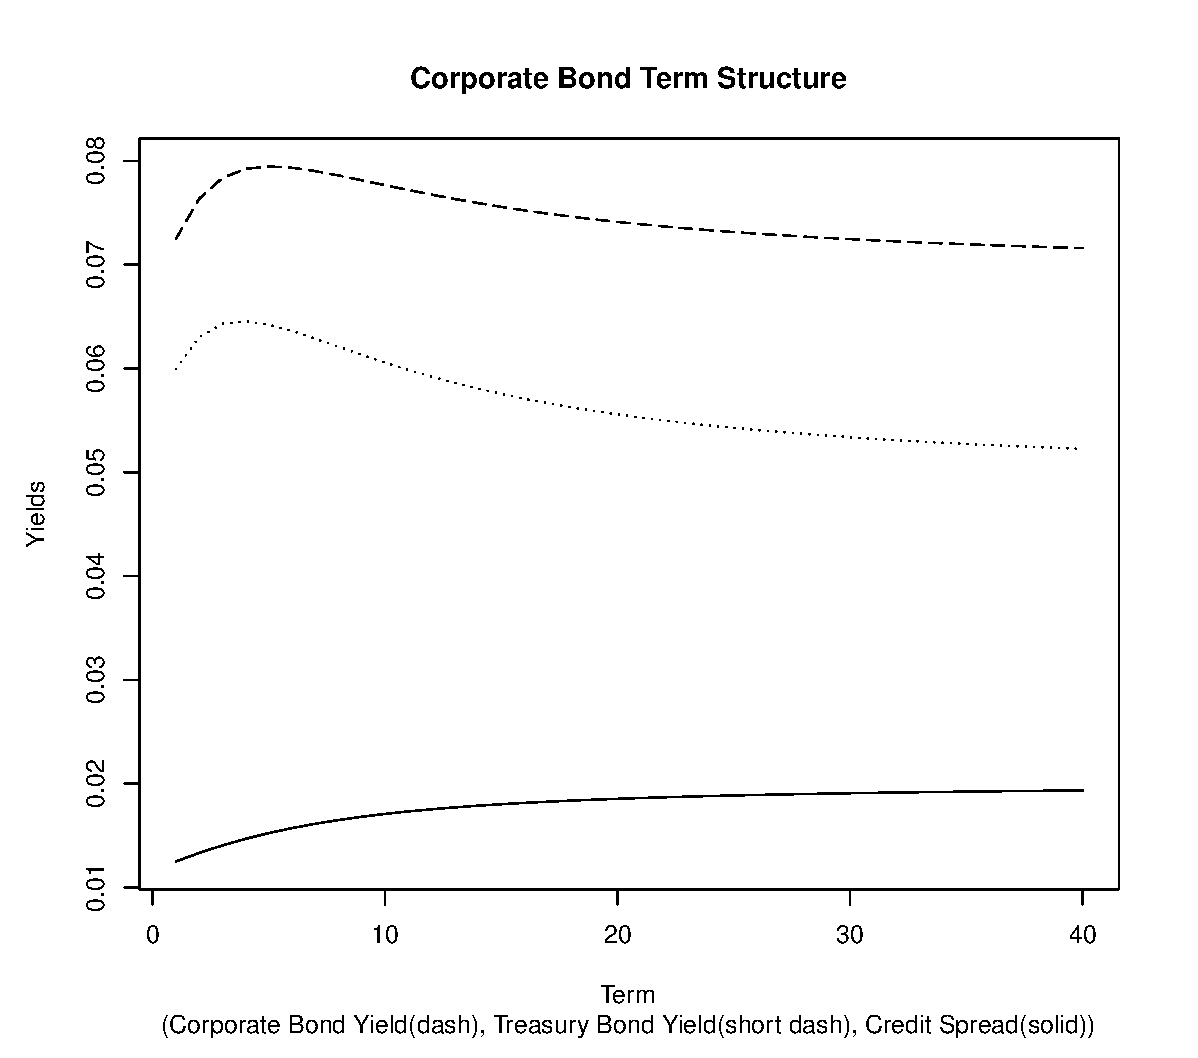
\epsfig{file=CorporateBondTermStructure.eps,height=8.cm,width=14.50cm}
\end{center}
\begin{center}
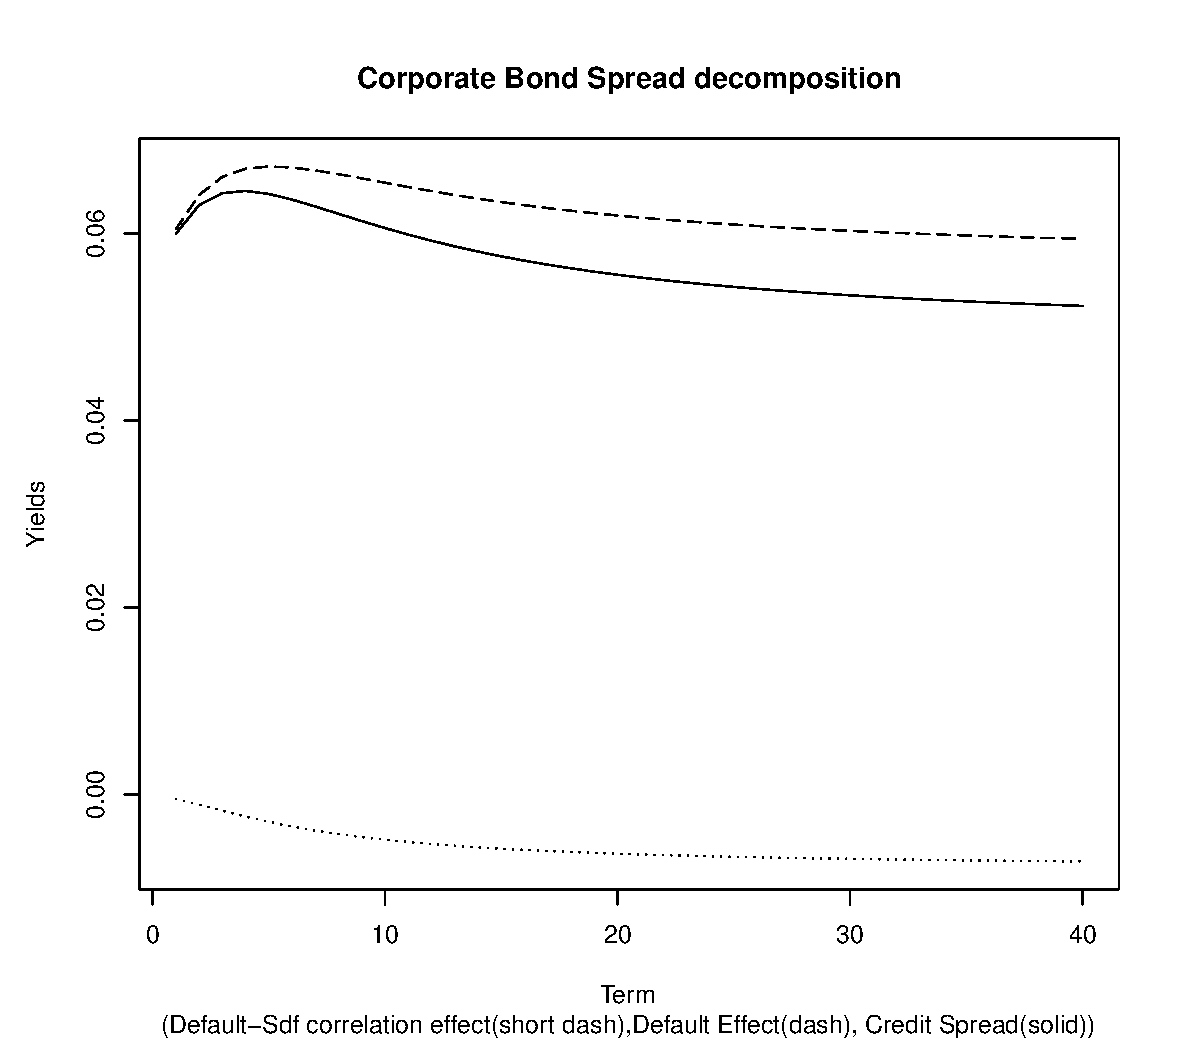
\epsfig{file=CorporateBondDecomposition.eps,height=8.cm,width=14.50cm}
\end{center}
On constate que la forme bossel�e typique des rendements d'obligation d'entreprise est facilement reproduite par le mod�le m�me avec des sensibilit�s constantes.
La d�composition du spread en un spread d'effet d�faut et un spread d'effet de corr�lation de d�faut-facteur d'escompte stochastique montre que le spread d'effet de corr�lation de d�faut-facteur d'escompte stochastique est n�gatif et petit en valeur absolue.
\begin{displaymath}
s_i(t,t+h)=\pi_i(t,t+h)+(s_i(t,t+h)-\pi_i(t,t+h))
\end{displaymath} 
\begin{displaymath}
s_i(t,t+h)-\pi_i(t,t+h)=-\log \left\{1+\frac{Cov_t (M_{t,t+1}1_{\tau_i >t+1})}{E_t(M_{t,t+1})E_t(1_{\tau_i >t+1})}\right\}
\end{displaymath} 
\subsection{R�sultats pour les paniers first-to-default}
\begin{center}
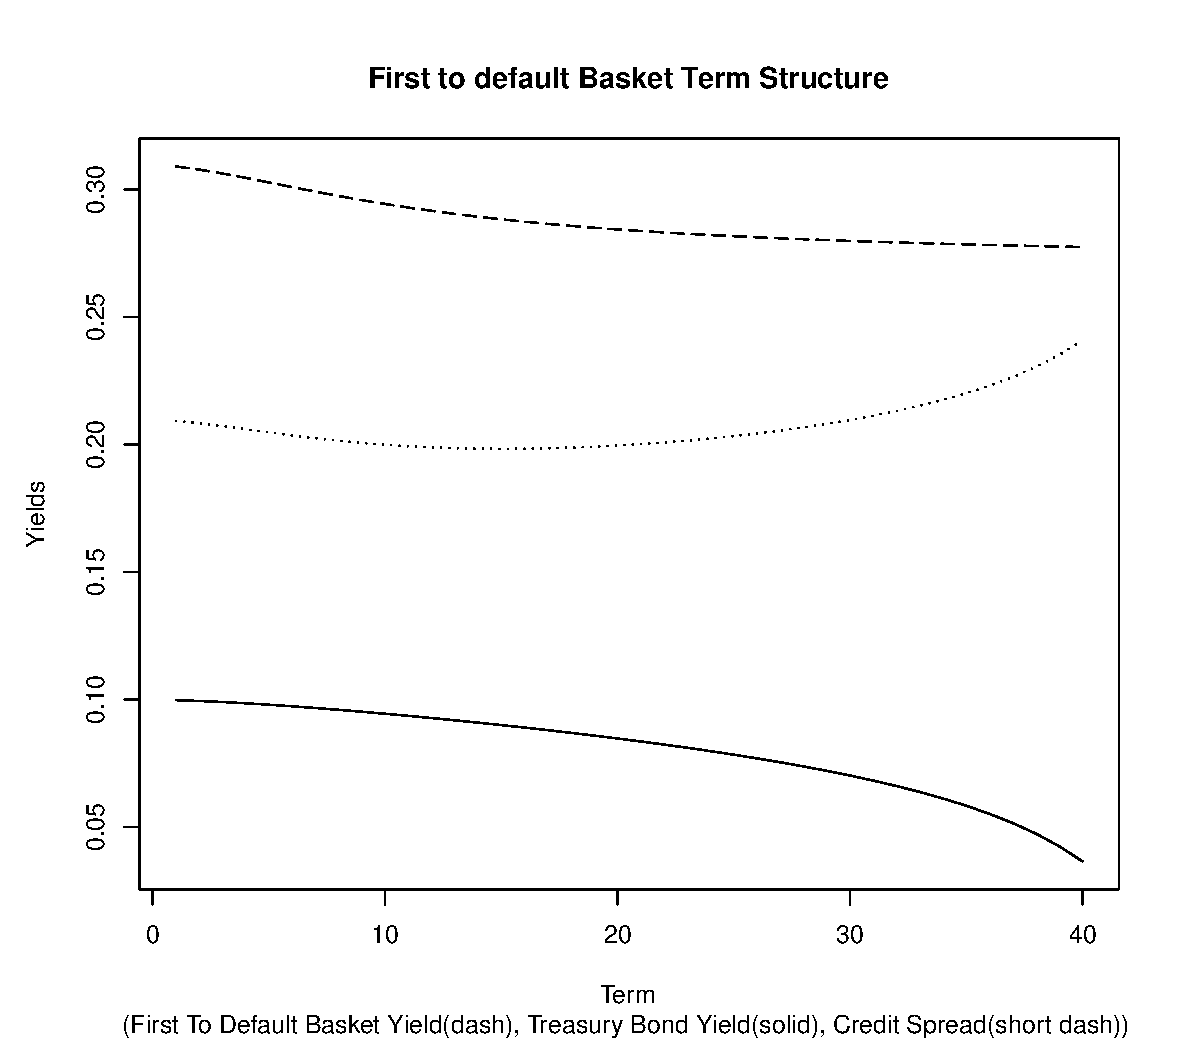
\epsfig{file=FirstToDefaultBasketTermStructure.eps,height=8.cm,width=14.50cm}
\end{center}
\begin{center}
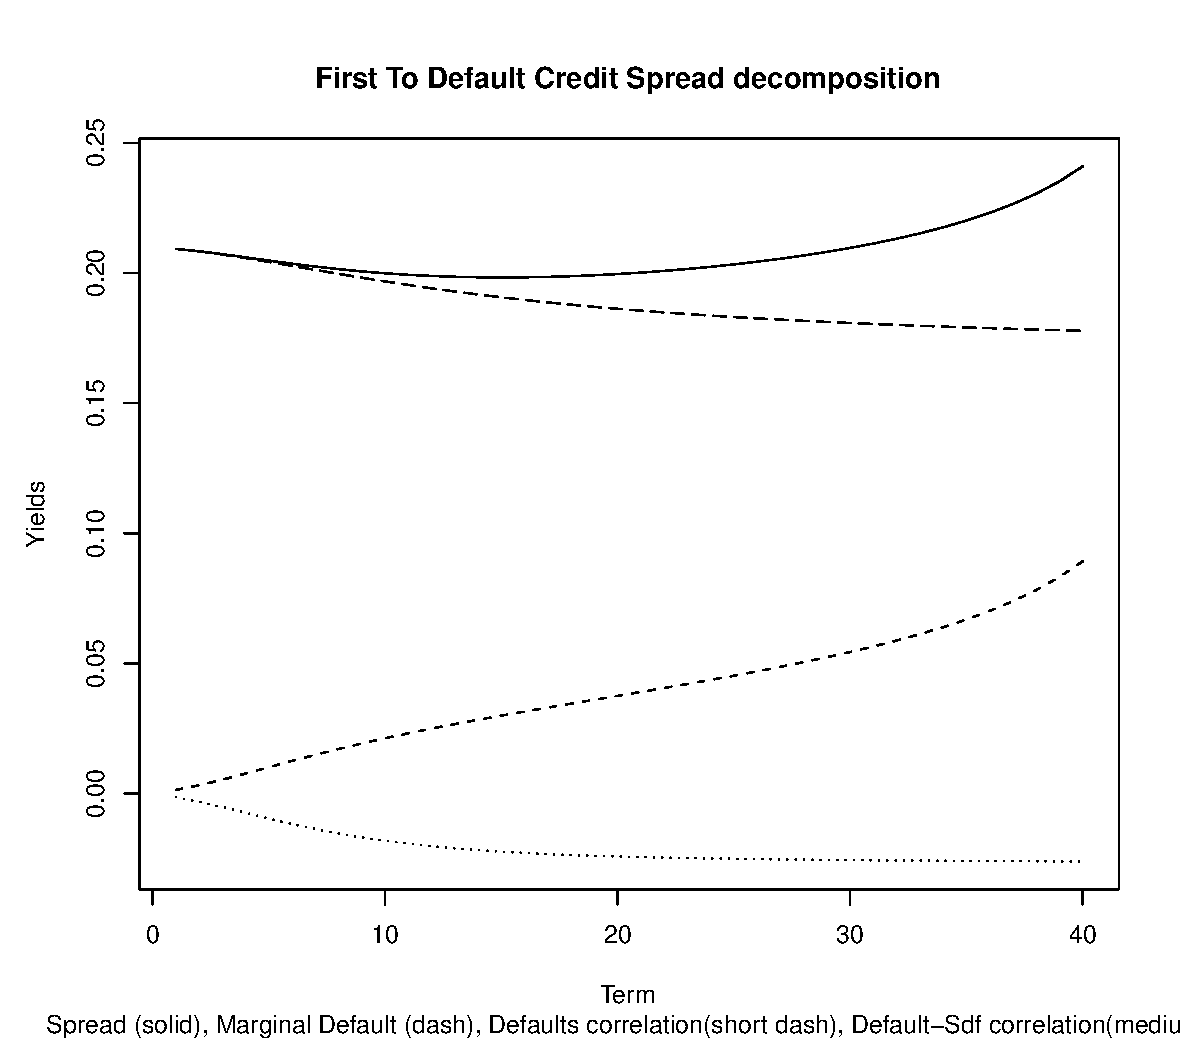
\epsfig{file=FirstToDefaultBasketDecomposition.eps,height=8.cm,width=14.50cm}
\end{center}
\begin{displaymath}
s(t,t+h)=\pi*(t,t+h)+(\pi(t,t+h)-\pi*(t,t+h))+(s(t,t+h)-\pi(t,t+h))
\end{displaymath} 
La composante principale de ce spread correspond � l'effet de d�faut marginal. La corr�lation de d�faut est n�gative, alors que la corr�lation d�faut-stochastic discount factor est positive.
\subsection{R�sultats pour les obligations d'entreprise avec des taux de recouvrement distincts}
\begin{center}
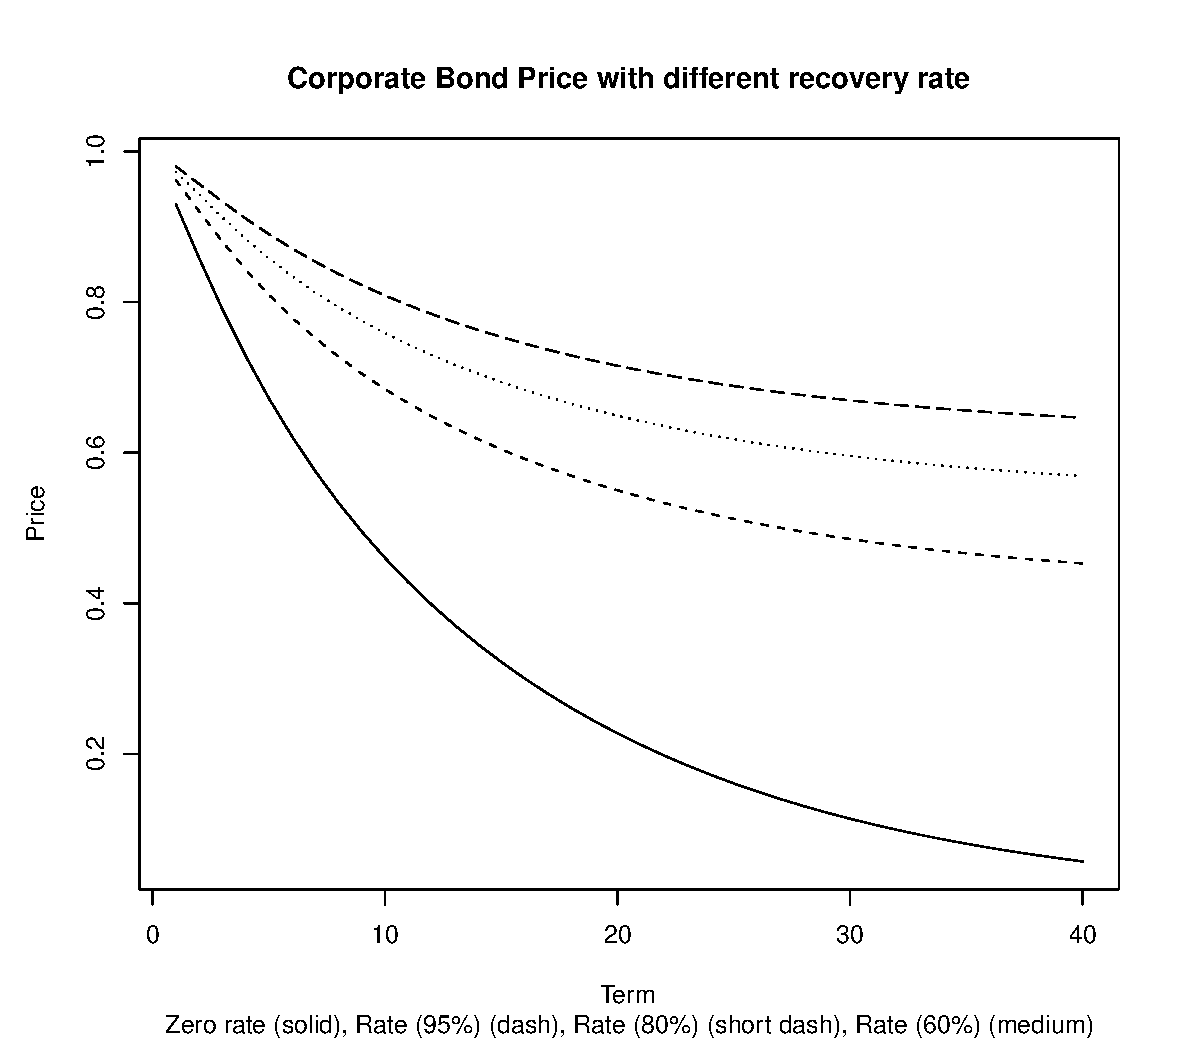
\epsfig{file=CorporateBondRecoveryPrice.eps,height=8.cm,width=14.50cm}
\end{center}
\begin{center}
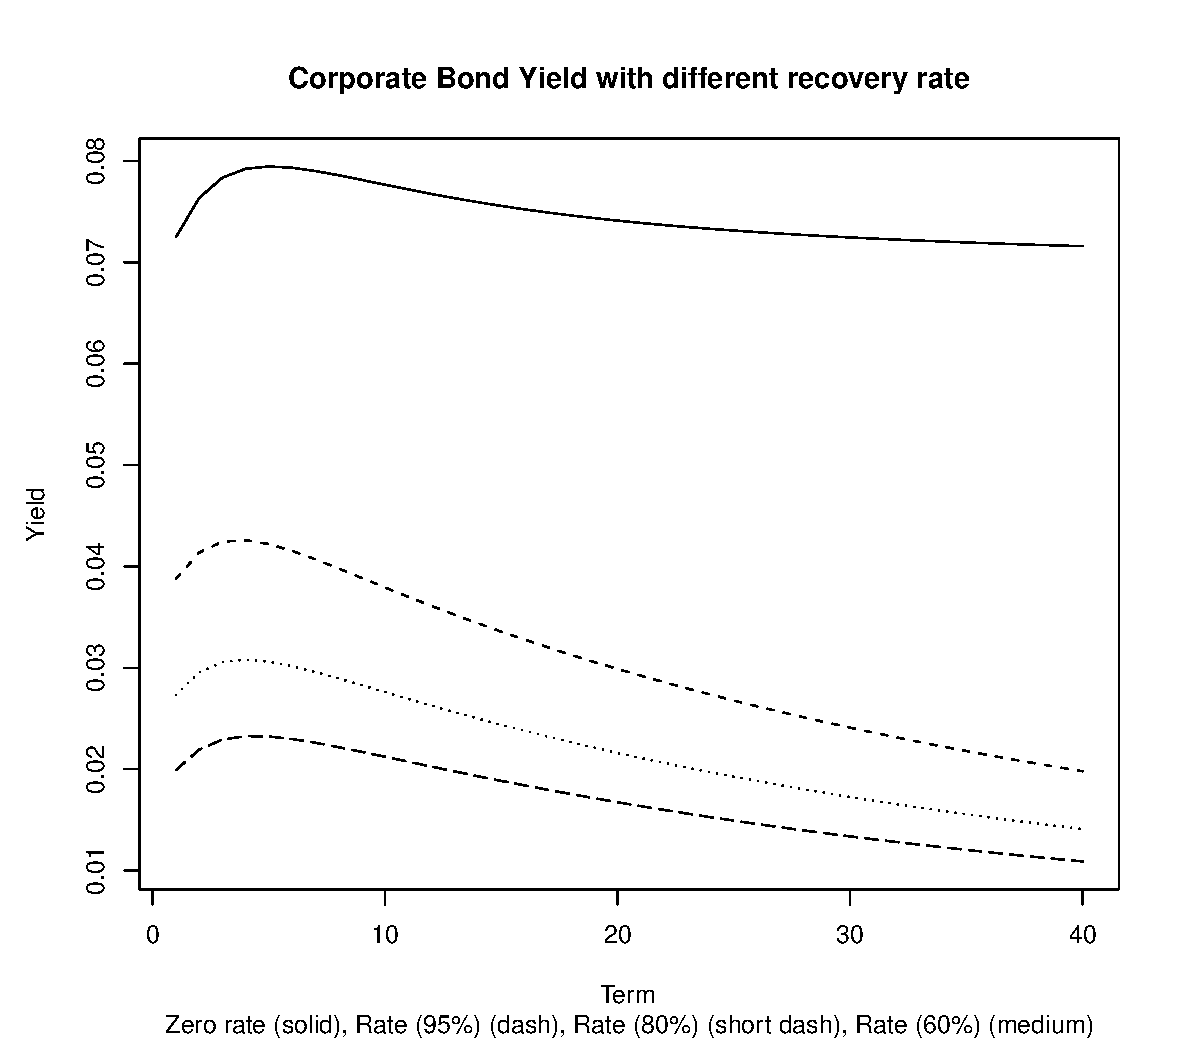
\epsfig{file=CorporateBondRecoveryYield.eps,height=8.cm,width=14.50cm}
\end{center}
\newpage
\begin{center}{\Huge Conclusion et Perspectives}
\end{center}
{\large
Ci-dessous la conclusion du rapport.
} 
\begin{thebibliography}{1}
\bibitem{MGP}
A. MONTFORT, C. GOUERIOUX et V. POLIMENIS.
\newblock{\em Affine models for credit risk analysis.}
\newblock Journal of Financial Econometrics, (2006), France.
\bibitem{JDG}
J. JASIAK, S. DAROLLES et C. GOUERIOUX.
\newblock{\em Compound autoregressive models.}
\newblock  (2002).
\end{thebibliography}
%\newpage
%\appendix
%\input{OperateursSurfaciques}
%\input{Sobolev}
%\input{ElementsFinisRappel}
%\include{RoutineVol}
\end{document}
